\documentclass[a4paper,12pt]{article}

\usepackage{abakos}
\usepackage{abntex2cite} 
\usepackage{tikz}
\usepackage{float}
\usepackage{amssymb} % Para \checkmark
\usepackage{amsmath} % Para \text em modo matemático

\usetikzlibrary{positioning,arrows.meta,shadows.blur,fit,calc} 

%%%%%%%%%%%%%%%%%%%%%%%%%%%
%Capa da revista
%%%%%%%%%%%%%%%%%%%%%%%%%%

%\setcounter{page}{80} %iniciar contador de pagina de valor especificado, quando o artigo for alocado a uma edição
\newcommand{\monog}{Personalização de Conteúdo Fitness em Rede Social por meio de um Sistema de Recomendação Híbrido}
\newcommand{\monogES}{Fitness Content Personalization in Social Networks through a Hybrid Recommender System}
\newcommand{\origem}{Brasil}
\newcommand{\editorial}{\textbf{Abakós}, Belo Horizonte, v. 8, n. 2, p. 00-00, Jul. 2021 - ISSN: 2316-9451}  % p. xx-xx – páginas inicial-final do artigo
% \newcommand{\lcc}{\scriptsize{Licença Creative Commons Attribution-NonCommercial-NoDerivs 3.0 Unported}}

%%%%%%%%%%%%%%%%%INFORMAÇÕES SOBRE AUTORES %%%%%%%%%%%%%%%%%%%%%%%%%%%%%%%
% Autor A
\newcommand{\AutorA}{Izabela Castanheira Galinari}
\newcommand{\funcaoA}{}
\newcommand{\cursA}{Engenharia de Computação}
\newcommand{\emailA}{izabela.galinari02@gmail.com}

% Autor B
\newcommand{\AutorB}{Philipi Gariglio Carvalho Faustino Altoe}
\newcommand{\funcaoB}{}
\newcommand{\cursB}{Engenharia de Computação}
\newcommand{\emailB}{philipigariglio@gmail.com}

% Autor C
\newcommand{\AutorC}{Raphael Lulli Duarte Tanos Galdino}
\newcommand{\funcaoC}{}
\newcommand{\cursC}{Engenharia de Computação}
\newcommand{\emailC}{raphaellulli@hotmail.com}

\newcommand{\AutorD}{Felipe Augusto Lara Soares}
\newcommand{\funcaoD}{}
\newcommand{\cursD}{Engenharia de Computação}
\newcommand{\emailD}{felipesoares@pucminas.br}

\newcommand{\keyword}[1]{\textsf{#1}}

\begin{document}

% %%%%%%%%%%%%%%%%%%%%%%%%%%%%%%%%%%
% %% Pagina de titulo
% %%%%%%%%%%%%%%%%%%%%%%%%%%%%%%%%%%

\begin{flushleft}
\begin{minipage} [c][5cm][b]{16.5cm} % Cabeçalho da primeira página da revista

\includegraphics[scale=1.1]{figuras/pucmg.png} 
\end{minipage}
 \vspace{0cm} { %Rodapé das páginas da revista
 \singlespacing \Large{\monog \symbolfootnote[1]{Submetido em DD/MM/AAAA - Aceito em DD/MM/AAAA} \\ }
  \normalsize{\monogES}
 }
\end{flushleft}

\begin{flushright}
\singlespacing
\normalsize{\AutorA \footnote{\funcaoA \cursA, \origem -- \emailA}} \\
\normalsize{\AutorB \footnote{\funcaoB \cursB, \origem -- \emailB}} \\
\normalsize{\AutorC \footnote{\funcaoC \cursC, \origem -- \emailC}} \\
\normalsize{\AutorD \footnote{\funcaoD \cursD, \origem -- \emailD}} \\
\end{flushright}
\thispagestyle{empty}

\begin{abstract}
\noindent
A prática insuficiente de atividade física permanece um desafio relevante de saúde pública, exigindo intervenções capazes de engajar a população. Em ambientes digitais, o excesso de informação dificulta a descoberta de conteúdos adequados ao perfil e momento de cada usuário, tornando os sistemas de recomendação ferramentas essenciais para a personalização. Diante disso, este trabalho apresenta o desenvolvimento e a avaliação de um sistema de recomendação voltado à personalização de conteúdo sobre atividade física em uma rede social. A proposta utiliza como base experimental a base de dados LDBC SNB, da qual são extraídos posts, interações, interesses declarados e relações sociais associados a esse domínio. Sobre esses dados, foi estruturado um fluxo reproduzível de preparação, separação em treino, validação e teste, treinamento e avaliação. O sistema de recomendação combina sinais de similaridade de conteúdo, coocorrência de \textit{tags}, recência, popularidade e influência do grafo social em um modelo híbrido de referência explicável, além de incluir uma trilha de aprendizado para ranqueamento (\textit{Learning to Rank}) com \textit{LightGBMRanker} para comparação entre modelos. \textcolor{green}{Acho que essa parte pode ser tirada: A avaliação é organizada por meio de uma comparação entre múltiplos modelos, considerando métricas de ranqueamento e indicadores complementares de cobertura, diversidade, novidade e latência. Como principal contribuição, o trabalho consolida uma arquitetura experimental rastreável para o estudo da recomendação de conteúdo \textit{fitness} em contexto social, permitindo comparar abordagens de ranqueamento sob um mesmo protocolo de dados e avaliação.}
Os resultados mostraram que o \textit{baseline} híbrido obteve o melhor NDCG@10 (0,0023 em \texttt{SF3}), enquanto o \textit{LightGBMRanker} liderou no NDCG@100 (0,0082) e na avaliação manual qualitativa (9/12 critérios atendidos).
\\\textbf{\keyword{Palavras-chave: }}Sistemas de Recomendação, Aprendizado para Ranqueamento, Grafo Social, Atividade Física
\end{abstract}

%%%%%%%%%%%%%%%%%%%%%%%%%%%%%%%%%%%%%%%%%%%%%%%%%%%%%%%%%
\newpage 
\selectlanguage{english}
\begin{abstract}
\noindent
This work presents the development and evaluation of a recommender system aimed at personalizing fitness-related content in a social network. The proposal uses the LDBC SNB dataset as its experimental basis, from which posts, interactions, declared interests, and social relationships associated with physical activity are extracted. On top of these data, a reproducible pipeline was structured for data preparation, train-validation-test splitting, training, and evaluation. The recommender combines content similarity, tag co-occurrence, recency, popularity, and social graph influence in an explainable hybrid baseline, while also including a Learning to Rank track with LightGBMRanker for model comparison. Results showed that the hybrid baseline achieved the best NDCG@10 (0.0023 on \texttt{SF3}), while the LightGBMRanker led in NDCG@100 (0.0082) and in the qualitative manual evaluation (9/12 criteria met).
\\\textbf{\keyword{Keywords: }}Recommendation Systems, Learning to Rank, Social Graph, Physical Activity
\end{abstract}

\newpage

\selectlanguage{brazilian}
 \onehalfspace  % espaçamento 1.5 entre linhas
 \setlength{\parindent}{1.25cm}

%%%%%%%%%%%%%%%%%%%%%%%%%%%%%%%%%%%%%%%%%%%%%%%%%
%% INICIO DO TEXTO
%%%%%%%%%%%%%%%%%%%%%%%%%%%%%%%%%%%%%%%%%%%%%%%%%

\section{Introdução}
A prática insuficiente de atividade física permanece um desafio relevante de saúde pública no Brasil, contribuindo para o aumento de doenças crônicas não transmissíveis. Dados do \citeonline{Vigitel2023} indicam que os níveis de atividade física observados nas capitais brasileiras ainda demandam políticas e estratégias capazes de reduzir o sedentarismo e ampliar a adoção de rotinas ativas. Em paralelo, a Organização Mundial da Saúde recomenda, para adultos, entre 150 e 300 minutos semanais de atividade aeróbica moderada, parâmetro que ainda não é alcançado por parcela expressiva da população \cite{WHO2020}.

Nesse cenário, intervenções digitais voltadas ao acompanhamento e ao estímulo da atividade física vêm recebendo atenção crescente, sobretudo quando buscam adaptar conteúdos ao contexto do usuário \cite{Agans2025PARecommender,Venka2022CARS}. Contudo, a simples disponibilização de conteúdos em plataformas digitais não garante que cada pessoa receba informações compatíveis com seus interesses, seu momento de uso e sua realidade social.

Em ambientes com grande volume de itens e interações, essa adaptação depende de mecanismos capazes de selecionar e ordenar conteúdos segundo critérios de relevância \cite{10.1145/3285029}. É nesse ponto que se inserem os sistemas de recomendação, entendidos neste trabalho como mecanismos computacionais voltados à seleção e ao ranqueamento de itens potencialmente mais relevantes para cada usuário.

Em serviços digitais, esses sistemas exercem papel estratégico na organização da informação \cite{GomezUribe2016Netflix}. No domínio da atividade física, sua utilidade tende a crescer quando também consideram sinais sociais, uma vez que interações entre pares podem influenciar comportamento e engajamento \cite{Franken2023}.

Diante desse problema, este trabalho propõe o desenvolvimento e a avaliação de um sistema de recomendação para uma rede social voltada à atividade física. O estudo utiliza dados extraídos do LDBC SNB \cite{Angles2020LDBCSNB} e organiza um fluxo com as etapas de coleta, preparação, treinamento, validação e avaliação dos modelos. Como contribuição técnica, foi desenvolvido o aplicativo FitConnect, que serve como ambiente de interação e estudo de caso para a coleta de sinais e experimentações. Desse modo, o problema investigado neste trabalho não se limita à oferta de conteúdo, mas à construção de um processo de ordenação que articule conteúdo, contexto temporal e relações sociais.

A solução investigada é construída em etapas. Primeiramente, o sistema combina similaridade de conteúdo, coocorrência de marcadores temáticos (\textit{tags}), recência, popularidade e informação do grafo social em um modelo híbrido de referência, onde cada sinal possui um peso interpretável. Em complemento, o trabalho incorpora uma trilha de aprendizado para ranqueamento (\textit{Learning to Rank}), permitindo que a importância de cada um desses sinais seja aprendida automaticamente a partir dos dados. A contribuição central do trabalho consiste em estruturar e comparar, em um mesmo ambiente experimental, essas diferentes abordagens de recomendação para apoiar a personalização de conteúdos sobre atividade física.

O restante do trabalho está organizado da seguinte forma: a Seção 2 apresenta a fundamentação teórica sobre inteligência artificial, sistemas de recomendação e métricas de avaliação; a Seção 3 discute os trabalhos correlatos; a Seção 4 descreve a metodologia adotada, com destaque para materiais e método; a Seção 5 apresenta os experimentos e resultados; e, por fim, a Seção 6 apresenta a conclusão do trabalho.





\section{Fundamentação Teórica}

Esta seção apresenta os conceitos centrais que sustentam a proposta desenvolvida no trabalho. 

\subsection{Inteligência Artificial e Sistemas de Recomendação}

% No contexto deste trabalho, 

A Inteligência Artificial é compreendida como o conjunto de métodos computacionais utilizados para apoiar decisões automáticas a partir de dados. Entre essas aplicações, os sistemas de recomendação ocupam papel relevante por permitirem selecionar e ordenar conteúdos potencialmente mais úteis para cada usuário em ambientes com grande volume de informação \cite{10.1145/3285029,GomezUribe2016Netflix}.

Em termos gerais, um sistema de recomendação busca estimar a relevância de itens, como filmes, músicas, produtos ou publicações, com base em sinais observáveis do contexto, do conteúdo e do comportamento dos usuários. No cenário da atividade física, revisões recentes indicam que esses sistemas podem contribuir para tornar intervenções digitais mais aderentes ao perfil e ao momento de uso de cada pessoa \cite{Venka2022CARS,Agans2025PARecommender}.

Para atingir esse objetivo, diferentes estratégias de filtragem podem ser empregadas. A filtragem baseada em conteúdo parte das características do próprio item recomendado. Em vez de depender exclusivamente do comportamento coletivo dos usuários, ela compara descritores dos itens com o perfil de interesse do usuário ou com a descrição do item de referência. Por outro lado, a filtragem colaborativa procura identificar padrões de interesse a partir do comportamento agregado de diferentes usuários. Sua ideia central é que interações passadas podem revelar relações úteis entre usuários, itens ou grupos de itens, permitindo inferir preferências prováveis mesmo quando os conteúdos não são idênticos \cite{10.1145/3285029}.

Quando essas abordagens são utilizadas em conjunto, formam-se os modelos híbridos. Esses modelos combinam diferentes fontes de evidência em um mesmo processo de recomendação. Essa estratégia é relevante porque permite articular características do conteúdo, padrões coletivos de interação e informações contextuais em uma única função de ranqueamento \cite{Venka2022CARS}. Uma variação dessa abordagem é o modelo híbrido de referência explicável, que designa uma arquitetura em que cada sinal possui significado claro e contribuição interpretável no cálculo do \textit{score} final.


\subsection{Sinais de ranqueamento}

Como a recomendação não depende de um único critério de relevância, múltiplos sinais podem ser utilizados para ordenar os candidatos. A combinação desses sinais forma a base de modelos híbridos e de algoritmos de aprendizado \cite{10.1145/3285029}.

Similaridade de conteúdo é o grau de proximidade temática entre dois itens. Quando dois \textit{posts} compartilham marcadores semânticos semelhantes, entende-se que tratam de assuntos próximos, o que aumenta a chance de um deles ser relevante para quem demonstrou interesse no outro \cite{Lops2011CB}.

Coocorrência de \textit{tags} corresponde à frequência com que determinados marcadores aparecem juntos em um mesmo conjunto de dados. Quando duas \textit{tags} surgem repetidamente associadas nas publicações, essa relação pode ser explorada como indício de proximidade temática ou comportamental. Assim, a coocorrência amplia a recomendação para além da coincidência exata de marcadores, permitindo recuperar conteúdos relacionados.

Recência é o sinal temporal que favorece itens mais recentes ou mais próximos do momento de referência da consulta. Em plataformas dinâmicas, a relevância de um conteúdo não depende apenas do tema, mas também de sua posição no tempo. Por isso, modelos de recomendação frequentemente incorporam mecanismos de decaimento temporal para reduzir o peso de conteúdos muito antigos em relação ao contexto atual \cite{Koren2009Temporal}.

Popularidade representa o interesse coletivo acumulado em torno de um item ou de um grupo de itens. Em termos práticos, ela pode ser estimada por volume de interações, frequência de acesso ou intensidade de engajamento. Esse sinal funciona como evidência complementar de relevância, especialmente útil quando se deseja considerar o comportamento agregado da comunidade \cite{Covington2016YouTube}.

Por fim, a influência do grafo social é a representação das relações entre usuários na forma de nós e conexões. Quando esse tipo de estrutura é incorporado à recomendação, torna-se possível considerar não apenas o conteúdo consumido, mas também a posição social de quem interage com ele. Em redes sociais voltadas à atividade física, interações entre pares podem influenciar engajamento e comportamento, o que justifica o uso de sinais associados à estrutura social no processo de ranqueamento \cite{Franken2023}.

Em um modelo híbrido de referência explicável, o \textit{score} final do item pode ser entendido como uma combinação ponderada desses componentes:

\begin{equation}
\label{eq:score_hibrido}
score(i,q) = w_c \cdot s_{c} + w_o \cdot s_{o} + w_r \cdot s_{r} + w_s \cdot s_{s} + w_p \cdot s_{p}
\end{equation}

\noindent onde, $score(i,q)$ é a pontuação final de relevância do item $i$ para a consulta $q$; $w_c, w_o, w_r, w_s, w_p$ são os pesos atribuídos a cada sinal, cuja soma é igual a 1; $s_{c}$ é o \textit{score} de similaridade de conteúdo (cálculo de cosseno entre vetores de \textit{tags}); $s_{o}$ é o \textit{score} de coocorrência de \textit{tags}; $s_{r}$ é o \textit{score} de recência (decaimento temporal); $s_{s}$ é o \textit{score} de influência do grafo social; $s_{p}$ é o \textit{score} de popularidade histórica do item.

\subsection{Aprendizado para ranqueamento}

Ranquear significa ordenar itens de acordo com um critério de relevância. Em muitos problemas de recomendação, não basta decidir se um item é potencialmente adequado; é necessário determinar também em que posição ele deve aparecer para o usuário. O Aprendizado para Ranqueamento (do inglês \textit{Learning to Rank}), corresponde à família de métodos supervisionados que aprendem essa ordenação a partir de exemplos previamente observados \cite{Burges2010LTROverview}.

Diferentemente de um modelo com pesos definidos manualmente, o \textit{Learning to Rank} busca estimar, a partir dos dados, como cada atributo deve influenciar a ordem final dos itens. Em aplicações de recomendação, isso permite aprender combinações mais ajustadas entre sinais de conteúdo, interação e contexto, reduzindo a dependência de calibração exclusivamente manual.

O \textit{LightGBMRanker} é um algoritmo específico utilizado em tarefas de ranqueamento, baseado em árvores de decisão com aumento de gradiente (\textit{Gradient Boosting Decision Trees}). Ele é projetado para otimizar métricas de ordenação de forma eficiente, permitindo que a importância relativa de diversos atributos seja aprendida diretamente a partir dos dados de treinamento \cite{Ke2017LightGBM}.

Em tarefas de ranqueamento, a avaliação precisa considerar não apenas se um item relevante foi recuperado, mas também a posição em que ele aparece na lista. Por essa razão, métricas de ordenação são particularmente importantes na análise de sistemas de recomendação. A \textit{Normalized Discounted Cumulative Gain} (\textit{NDCG}) permite avaliar se os itens mais relevantes estão concentrados nas primeiras posições da lista \cite{Jarvelin2002NDCG}. Ela atribui pesos maiores aos acertos no topo da lista e penaliza acertos em posições inferiores. Já a \textit{Mean Reciprocal Rank} (\textit{MRR}) enfatiza quão cedo surge o primeiro item relevante para cada consulta \cite{Craswell2009MRR}, sendo calculada pelo inverso da posição do primeiro acerto. Ambas as métricas são fundamentais para mensurar a eficácia de algoritmos de ranqueamento, especialmente em cenários onde a atenção do usuário é limitada aos primeiros resultados.




\section{Trabalhos Correlatos}


Em plataformas digitais de grande escala, os sistemas de recomendação deixaram de ser um recurso complementar e passaram a ocupar posição central na interação com o usuário \cite{10.1145/3285029}. \citeonline{GomezUribe2016Netflix} mostram, no caso da Netflix, que a recomendação está diretamente associada à organização personalizada do catálogo, ao engajamento de médio prazo e à retenção dos usuários, sendo continuamente aprimorada por meio de testes A/B e de dados históricos de interação.

No domínio de sistemas de recomendação aplicados à atividade física, \citeonline{Venka2022CARS} apresentam uma revisão sobre algoritmos de Inteligência Artificial sensíveis ao contexto em recomendadores para \textit{fitness}. Os autores mostram que fatores como preferências individuais, contexto de uso e dados comportamentais podem ampliar a pertinência das recomendações, ao mesmo tempo em que evidenciam a necessidade de soluções mais bem adaptadas a cenários reais de uso.

Já \citeonline{Zhao2020PersonalizedFitness} propõem um sistema de assistência fitness que fornece recomendações personalizadas de atividades físicas, a partir de modelagem dinâmica de usuários. No estudo, os autores acompanharam 40 participantes por 60 dias e observaram diferenças estatisticamente significativas em motivação e preferência entre os grupos avaliados, indicando que a combinação entre personalização e gamificação pode contribuir positivamente para o engajamento em atividades físicas. Esse correlato mostra, de forma mais direta, como um sistema de recomendação pode atuar no domínio do fitness.

Também em direção semelhante, \citeonline{Agans2025PARecommender} investigam o uso de tecnologia de recomendação para apoiar a adoção de atividade física entre jovens inativos com maior peso corporal. O estudo desenvolveu um sistema capaz de sugerir atividades com base em dados populacionais e avaliou o interesse dos participantes em utilizar esse tipo de recomendação. Os resultados indicaram que aproximadamente metade dos participantes demonstrou disposição para utilizar o sistema, e parte daqueles que receberam sugestões, efetivamente experimentou as atividades recomendadas. O trabalho reforça o potencial de sistemas de recomendação para apoiar a descoberta de práticas físicas mais compatíveis com perfis e preferências individuais.

Em redes sociais, a recomendação também pode explorar explicitamente a estrutura relacional entre usuários. \citeonline{10457840} propõem um método de recomendação de participantes em redes sociais baseadas em eventos, considerando aspectos de relevância e equidade na ordenação. Embora o problema tratado seja distinto do presente trabalho, o estudo é pertinente por mostrar como informações de rede e de contexto social podem ser incorporadas ao processo de recomendação.

Em conjunto, esses trabalhos mostram que a literatura já reconhece a importância da personalização, do contexto e das relações sociais em sistemas de recomendação. A proposta desenvolvida neste trabalho, aproxima-se dessa linha ao tratar a recomendação como núcleo técnico do sistema, mas se diferencia por direcionar o problema para a ordenação de conteúdo sobre atividade física em rede social, explorando sinais de conteúdo, coocorrência, recência, popularidade e grafo social em um mesmo ambiente experimental. Além disso, o trabalho compara um modelo híbrido de referência com uma trilha de aprendizado para ranqueamento, o que amplia a análise para além de uma única estratégia de recomendação.




\section{Metodologia}

Esta seção apresenta os materiais empregados no estudo e o método adotado para desenvolver, treinar e comparar os modelos de recomendação. O foco recai sobre o fluxo de dados e sobre as escolhas metodológicas associadas ao sistema de recomendação, que atua como o motor de personalização do aplicativo FitConnect.


\subsection{Materiais}

A base de dados utilizada foi o LDBC Social Network Benchmark (\textit{LDBC SNB}) \cite{Angles2020LDBCSNB}, empregado como fonte de posts, comentários, \textit{tags}, interações, interesses declarados e relações sociais. A partir da versão completa da base, foram extraídos apenas os registros associados ao domínio da atividade física, produzindo arquivos em formato \textit{parquet}, que é um formato de armazenamento de dados colunar otimizado para comprimir dados de forma eficiente, permitindo leitura rápida de colunas específicas.

O ambiente computacional do projeto foi organizado principalmente em Python 3.11. Na etapa de extração e transformação dos dados brutos, utilizou-se o DuckDB, um sistema de gerenciamento de banco de dados analítico em memória, ideal para processamento rápido de grandes volumes de dados. Complementarmente, foram utilizadas as bibliotecas pandas, NumPy e PyArrow para manipulação e estruturação dos dados. Para a construção do modelo híbrido de referência, empregou-se a biblioteca scikit-learn \cite{pedregosa2011scikit}, especialmente na vetorização binária das \textit{tags}. Para a trilha de aprendizado para ranqueamento, utilizou-se o \textit{LightGBMRanker}, disponibilizado na biblioteca LightGBM \cite{Ke2017LightGBM}. Para gerar uma representação semântica densa das \textit{tags} -- usada como atributo adicional pelo \textit{LightGBMRanker} --, empregou-se a biblioteca \textit{sentence-transformers}, com o modelo pré-treinado \texttt{all-MiniLM-L6-v2}, que produz vetores de 384 dimensões a partir dos nomes das \textit{tags}.

Como materiais intermediários do estudo, foram produzidos artefatos derivados da base inicial e os conjuntos de treino, validação e teste. Esses arquivos compõem a base efetiva sobre a qual os modelos são treinados e avaliados. Entre os principais artefatos, destacam-se:

\begin{itemize}
    \item[a)] \texttt{messages\_fitness.parquet}: contém os metadados de todas as publicações e comentários filtrados para o domínio fitness, incluindo data de criação, tamanho do texto e \textit{tags} associadas.
    \item[b)] \texttt{interactions\_fitness.parquet}: registra as ações dos usuários sobre os conteúdos, como curtidas, criação de posts e respostas, essenciais para inferir preferências.
    \item[c)] \texttt{tag\_cooccurrence.parquet}: armazena a frequência com que pares de \textit{tags} aparecem juntos nas publicações, servindo de base para o cálculo de similaridade semântica.
    \item[d)] \texttt{posts\_metadata.parquet}: versão consolidada dos dados dos posts, preparada especificamente para a etapa de treinamento dos modelos.
    \item[e)] \texttt{social\_scores.parquet}: contém os escores de influência calculados a partir do grafo social, indicando o peso das interações da rede de contatos para cada post.
    \item[f)] \texttt{user\_tag\_profile.parquet}: representa o perfil de interesse de cada usuário, construído a partir de suas interações históricas com diferentes \textit{tags}.
\end{itemize}

Além disso, o processo experimental foi padronizado por um orquestrador e por configurações parametrizáveis. Esses componentes permitem controlar hiperparâmetros de treinamento, famílias de modelo, etapas de avaliação e diretórios de saída, garantindo a reprodutibilidade dos experimentos.

\subsection{Versões da base utilizadas}
\label{subsec:versoes_base}

O \textit{LDBC SNB} disponibiliza diferentes versões da mesma rede social simulada, controladas por um parâmetro chamado \textit{scale factor} (SF), que multiplica de forma proporcional a quantidade de usuários, mensagens e interações geradas. Versões com SF maior produzem volumes muito superiores de dados, mantendo a mesma distribuição estatística e o mesmo esquema relacional. Para este trabalho, três versões da base foram utilizadas, com o objetivo de observar o comportamento dos modelos em diferentes ordens de grandeza, desde uma amostra de validação do protocolo até a versão final em escala maior.

A Tabela \ref{tab:rodadas_execucao_tcc} apresenta as três versões empregadas, junto com o volume bruto do arquivo compactado e o volume já filtrado para o domínio \textit{fitness}.

\begin{table}[H]
\centering
\caption{Versões da base \textit{LDBC SNB} utilizadas no estudo}
\label{tab:rodadas_execucao_tcc}
\small
\begin{tabular}{|p{1.6cm}|p{1.2cm}|p{1.6cm}|p{1.8cm}|p{2.2cm}|p{3.4cm}|}
\hline
\textbf{Rodada} & \textbf{Versão} & \textbf{Arquivo (\texttt{.tar.zst})} & \textbf{Mensagens \textit{fitness}} & \textbf{Interações \textit{fitness}} & \textbf{Objetivo} \\
\hline
Inicial & \texttt{SF0.1} & 18 MB & 38 & 94 & Fluxo completo validado e primeira leitura comparativa concluída. \\
\hline
Intermediária & \texttt{SF3} & 690 MB & 2.199 & 10.720 & Verificar o comportamento das métricas com maior volume de dados. \\
\hline
Final & \texttt{SF30} & 7,32 GB & 23.485 & 120.807 & Consolidar os resultados a serem apresentados na versão final do TCC. \\
\hline
\end{tabular}
\end{table}

A coluna \textbf{Arquivo (\texttt{.tar.zst})} refere-se ao volume do arquivo bruto comprimido disponibilizado pelo \textit{LDBC SNB}; as colunas \textbf{Mensagens \textit{fitness}} e \textbf{Interações \textit{fitness}} referem-se ao volume já restrito ao domínio do estudo após a aplicação dos filtros descritos na Seção de Método. Quando uma versão específica é mencionada ao longo do texto (por exemplo, \texttt{SF0.1}, \texttt{SF3} ou \texttt{SF30}), os números desta tabela podem ser consultados como referência.

\subsection{Método}

O método desenvolvido foi organizado em quatro etapas principais: Etapa 1: extração e preparação dos dados; Etapa 2: separação experimental; Etapa 3: treinamento dos modelos; e Etapa 4: avaliação e rastreabilidade. A Figura \ref{fig:fluxograma_metodologia} ilustra o fluxo de dados desde a base bruta até a avaliação dos modelos.

\begin{figure}[H]
\centering
\caption{Fluxograma do pipeline metodológico do sistema de recomendação.}
\label{fig:fluxograma_metodologia}
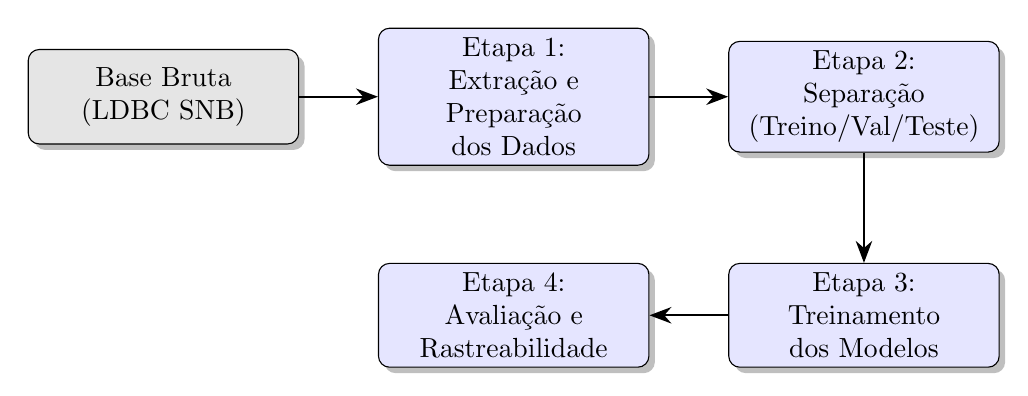
\begin{tikzpicture}[
    node distance=1.4cm and 1cm,
    box/.style={draw, rectangle, rounded corners, align=center, minimum width=3.4cm, minimum height=1.2cm, text width=3.2cm, fill=blue!10, drop shadow},
    arrow/.style={-{Stealth[scale=1.2]}, thick}
]

% Nodes
\node[box, fill=gray!20] (ldbc) {Base Bruta\\(LDBC SNB)};
\node[box, right=of ldbc] (extracao) {Etapa 1:\\Extração e Preparação\\dos Dados};
\node[box, right=of extracao] (split) {Etapa 2:\\Separação\\(Treino/Val/Teste)};
\node[box, below=of split] (treinamento) {Etapa 3:\\Treinamento\\dos Modelos};
\node[box, left=of treinamento] (avaliacao) {Etapa 4:\\Avaliação e\\Rastreabilidade};

% Arrows
\draw[arrow] (ldbc) -- (extracao);
\draw[arrow] (extracao) -- (split);
\draw[arrow] (split) -- (treinamento);
\draw[arrow] (treinamento) -- (avaliacao);

\end{tikzpicture}
\small \\ Fonte: Elaborado pelos autores.
\end{figure}

Em síntese, cada etapa do pipeline cumpre um papel distinto: a \textbf{Etapa 1} parte da base bruta do \textit{LDBC SNB} e produz os artefatos \textit{parquet} já restritos ao domínio \textit{fitness}, incluindo metadados de mensagens, contagens por \textit{tag}, escores de influência e perfis usuário-\textit{tag}; a \textbf{Etapa 2} divide as interações em treino, validação e teste segundo um corte temporal global; a \textbf{Etapa 3} treina o conjunto de modelos do \textit{benchmark} sobre o conjunto de treino, calibrando hiperparâmetros no conjunto de validação; e a \textbf{Etapa 4} realiza a avaliação \textit{offline} no conjunto de teste e registra o manifesto de execução para garantir rastreabilidade e reprodutibilidade.

\subsubsection{Etapa 1: Extração e preparação dos dados}

A primeira etapa consistiu em transformar uma base social genérica em um conjunto de dados orientado ao domínio da atividade física, já pronto para o treinamento. Para isso, o arquivo compactado do \textit{LDBC SNB} foi extraído e seus arquivos \textit{CSV} foram processados. Como a base original contém dados sobre diversos temas não relacionados ao escopo do trabalho, o conteúdo associado à temática \textit{fitness} foi identificado por duas estratégias complementares: correspondência por classes de \textit{tags} (ex: "sports", "health", "fitness") e filtragem direta pelos nomes das próprias \textit{tags} (ex: "running", "workout", "gym"). Esse procedimento resultou em tabelas com mensagens, interações, interesses e relações sociais já restritas ao domínio estudado.

A leitura e a filtragem dos arquivos \textit{CSV} brutos foram realizadas com o sistema analítico DuckDB, que permite executar consultas \textit{SQL} sobre arquivos em disco com baixo consumo de memória e alta velocidade. Sobre os resultados dessas consultas, foram aplicadas etapas adicionais de manipulação em \textit{Python} para preparar os artefatos finais: agregação das interações por \textit{post} e por usuário, montagem do perfil de afinidade entre usuário e \textit{tag}, cálculo dos escores de influência social a partir do grafo de amizades e construção das matrizes binárias de \textit{tags} por publicação. Também nessa etapa, os carimbos de tempo originais do \textit{LDBC SNB}, exportados como inteiros longos em milissegundos desde 1970, foram normalizados em uma coluna padronizada e preservados em todos os artefatos derivados. Esse cuidado garante que a ordem cronológica dos eventos seja preservada por todo o restante do \textit{pipeline}, condição fundamental para a etapa seguinte de separação dos dados.

Como resultado, são produzidos os principais artefatos próprios para treinamento e avaliação. Entre eles, destacam-se os metadados semânticos dos posts, a contagem de interações por \textit{tag}, os escores de influência social por post e os perfis usuário-\textit{tag}, todos serializados em formato \textit{parquet}.

Para ilustrar o impacto dessa filtragem, a Tabela \ref{tab:estatisticas_extracao} apresenta o volume de dados extraídos da versão SF0.1 do \textit{LDBC SNB} após a aplicação das regras de domínio.

Para tornar o processo mais claro, a Figura \ref{fig:fluxo_extracao} ilustra a lógica de alto nível dessa filtragem. O procedimento lê o \textit{dataset} bruto, identifica as \textit{tags} relevantes pelas regras de domínio, propaga essa seleção para \textit{posts} e comentários, e a partir daí restringe as interações e o grafo social associados.

\begin{figure}[H]
\centering
\caption{Fluxograma da etapa de extração e filtragem do conteúdo \textit{fitness}.}
\label{fig:fluxo_extracao}
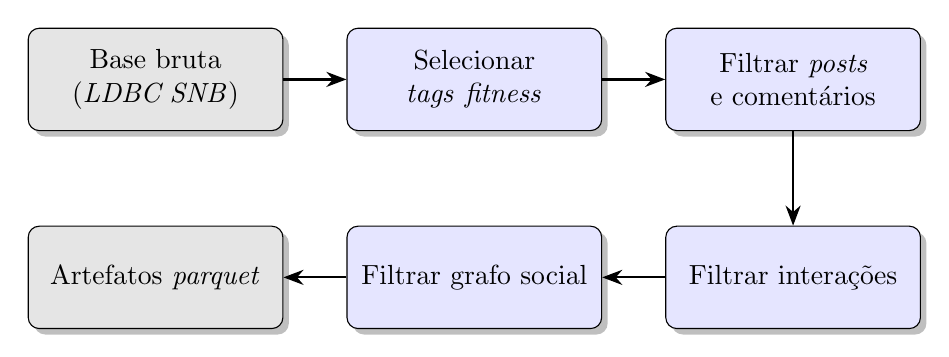
\begin{tikzpicture}[
    node distance=1.2cm and 0.8cm,
    box/.style={draw, rectangle, rounded corners, align=center, minimum width=3.2cm, minimum height=1.3cm, text width=3.0cm, fill=blue!10, drop shadow},
    iobox/.style={draw, rectangle, rounded corners, align=center, minimum width=3.2cm, minimum height=1.3cm, text width=3.0cm, fill=gray!20, drop shadow},
    arrow/.style={-{Stealth[scale=1.1]}, thick}
]

% Linha de cima (esquerda -> direita)
\node[iobox] (entrada) {Base bruta\\(\textit{LDBC SNB})};
\node[box, right=of entrada] (filtra_tags) {Selecionar \textit{tags} \textit{fitness}};
\node[box, right=of filtra_tags] (filtra_posts) {Filtrar \textit{posts} e comentários};

% Linha de baixo (direita -> esquerda)
\node[box, below=of filtra_posts] (filtra_int) {Filtrar interações};
\node[box, left=of filtra_int] (filtra_grafo) {Filtrar grafo social};
\node[iobox, left=of filtra_grafo] (saida) {Artefatos \textit{parquet}};

\draw[arrow] (entrada) -- (filtra_tags);
\draw[arrow] (filtra_tags) -- (filtra_posts);
\draw[arrow] (filtra_posts) -- (filtra_int);
\draw[arrow] (filtra_int) -- (filtra_grafo);
\draw[arrow] (filtra_grafo) -- (saida);

\end{tikzpicture}
\small \\ Fonte: Elaborado pelos autores.
\end{figure}

\begin{table}[H]
\centering
\caption{Estatísticas da base de dados após filtragem para o domínio \textit{fitness} (Versão \texttt{SF0.1})}
\label{tab:estatisticas_extracao}
\small
\begin{tabular}{|l|r|}
\hline
\textbf{Entidade} & \textbf{Volume após filtragem} \\
\hline
\textit{Tags} \textit{fitness} identificadas & 33 \\
Mensagens (\textit{Posts} e Comentários) & 158 \\
Interações (Curtidas, Respostas, Criações) & 381 \\
Interesses declarados por usuários & 7 \\
Arestas no grafo social & 7.973 \\
Pares de coocorrência de \textit{tags} & 0 \\
\hline
\end{tabular}
\end{table}

\subsubsection{Etapa 2: Separação experimental}

Na segunda etapa, as interações \textit{fitness} foram divididas em treino, validação e teste, nas proporções de 70\%, 15\% e 15\%, respectivamente. Esses três conjuntos têm finalidades complementares: o conjunto de treino é utilizado para ajustar os modelos, o conjunto de validação é empregado para calibrar pesos e hiperparâmetros, e o conjunto de teste permanece reservado exclusivamente para a avaliação final do desempenho \cite{Goodfellow2016DeepLearning,Hastie2001Elements}.

Em sistemas de recomendação, no entanto, o \emph{critério} da divisão é tão importante quanto a proporção. Diferentemente de problemas estáticos de classificação, em recomendação cada interação está associada a um instante específico no tempo, e o objetivo de produção é sempre o mesmo: prever, a partir do que o usuário já fez, o que ele provavelmente fará a seguir. Uma divisão puramente aleatória das interações, ou uma validação cruzada clássica (\textit{k-fold}), violaria essa estrutura, pois permitiria que o modelo fosse treinado com interações posteriores ao alvo de avaliação. Atributos derivados, como a coocorrência de \textit{tags}, a popularidade dos itens e os escores de influência social, representam o estado da rede em um determinado momento, e expô-los a interações futuras durante o treino caracterizaria vazamento de dados (\textit{data leakage}). Por essas razões, a separação adotada no estudo é \textbf{temporal global}.

O procedimento opera diretamente sobre o eixo cronológico padronizado na Etapa~1. As interações de todas as pessoas são ordenadas pelo carimbo de tempo e, sobre essa ordem global, são fixados dois cortes temporais que separam o estudo em três faixas contínuas. O primeiro corte, $t_{\text{train\_val}}$, marca o fim do conjunto de treino e o início da validação; o segundo, $t_{\text{val\_test}}$, marca o início do conjunto de teste. Assim, toda interação anterior a $t_{\text{train\_val}}$ é treino; entre os dois cortes, validação; e posterior a $t_{\text{val\_test}}$, teste. Os cortes são calculados de modo a respeitar as proporções 70\%/15\%/15\% e ficam registrados no manifesto da rodada para garantir reprodutibilidade.

O catálogo de \textit{posts} é mantido íntegro nos três conjuntos -- o que muda entre os conjuntos é apenas qual conjunto de \emph{interações} está disponível, refletindo o cenário real em que todos os itens existem no acervo, mas o histórico de cada usuário evolui ao longo do tempo. Em particular, as estatísticas derivadas (coocorrência de \textit{tags}, popularidade e influência social) são recalculadas usando exclusivamente as interações do treino, e a avaliação \textit{offline} sempre apresenta ao modelo um item de referência anterior ao corte de teste para predizer interações posteriores. Esse desenho preserva a coerência temporal do problema e produz métricas comparáveis ao desempenho que o sistema teria em produção.

\subsubsection{Etapa 3: Treinamento dos modelos}

Nesta etapa, três famílias de modelos foram desenvolvidas e treinadas para o sistema de recomendação, totalizando quatro configurações: um \textit{baseline} de popularidade, duas variantes de um modelo híbrido de referência e uma trilha de aprendizado para ranqueamento. Essa diversidade não é arbitrária: cada modelo responde a uma pergunta específica do estudo e estabelece um ponto de referência diferente para a comparação. A motivação, técnica e objetivo de cada um são descritos a seguir.

\paragraph{Popularidade (\textit{baseline} trivial)}

A primeira configuração é um recomendador de popularidade pura, que ignora qualquer informação sobre o usuário ou o contexto da consulta e devolve sempre os itens mais populares do catálogo. Esse tipo de baseline é classicamente recomendado na literatura de sistemas de recomendação como referência mínima para avaliar técnicas mais sofisticadas \cite{Lops2011CB}. Seu papel no estudo é funcionar como teste de sanidade do protocolo: se algum modelo elaborado perder para ele, há indício de problema na modelagem ou na avaliação. Não tem parâmetros de modelo nem etapa de treinamento.

\paragraph{\textit{Baseline} híbrido padrão (pesos manuais)}

Em seguida, foi implementado um modelo híbrido com pesos manuais sobre os cinco sinais centrais do estudo: similaridade de conteúdo, coocorrência de \textit{tags}, recência, popularidade e influência social. Modelos híbridos baseados em conteúdo desse tipo aproveitam metadados ricos do item, são interpretáveis e têm baixo custo computacional \cite{Lops2011CB}. Aqui, ele responde à pergunta de até que ponto uma heurística manual e explicável já consegue ser competitiva, sem qualquer ajuste sobre os dados.

\paragraph{\textit{Baseline} híbrido otimizado (pesos calibrados)}

A segunda variante do híbrido mantém os mesmos cinco sinais, mas os pesos passam a ser ajustados por busca em grade (\textit{grid search}) sobre o conjunto de validação, maximizando a métrica NDCG@10 \cite{Lops2011CB}. O objetivo é isolar o efeito da otimização: comparando essa variante com a anterior é possível medir, em isolamento, quanto ganho vem apenas de calibrar os pesos manuais, antes de introduzir qualquer modelo aprendido.

\paragraph{Aprendizado para ranqueamento (LightGBMRanker)}

A trilha de aprendizado para ranqueamento (\textit{Learning to Rank}, LTR) é representada por um \textit{LightGBMRanker} \cite{Ke2017LightGBM} treinado com objetivo \textit{lambdarank} \cite{Burges2010LTROverview}. O modelo aprende diretamente a função de ordenação a partir de pares \textit{query}-item gerados sobre o conjunto de treino, combinando os cinco sinais centrais do híbrido com atributos contextuais do item (sobreposição de \textit{tags}, número de \textit{tags}, comprimento do conteúdo, tipo de mensagem e idioma), com o perfil de afinidade do usuário e com atributos derivados de tempo e popularidade (diferença temporal entre item e consulta, popularidade em escala logarítmica, tamanho do histórico). Soma-se a esses atributos a \textit{tag\_embedding\_similarity}, um sinal contínuo de similaridade semântica entre o item de referência e o candidato, obtido pelo cosseno entre os vetores densos de 384 dimensões produzidos pelo encoder \texttt{all-MiniLM-L6-v2} a partir dos nomes das \textit{tags}. Essa \textit{feature} reconhece relações temáticas que a vetorização binária não captura, como a proximidade entre \textit{running} e \textit{jogging} ou entre \textit{strength} e \textit{lifting}. Para tornar o treino mais informativo, são amostrados exemplos negativos difíceis (\textit{hard negatives}) -- itens próximos da consulta mas não observados como relevantes -- e usados parâmetros conservadores de regularização (\texttt{min\_data\_in\_leaf}, \texttt{feature\_fraction}, \texttt{bagging\_fraction}). Essa trilha foi adotada para verificar em que medida a aprendizagem da ordenação consegue superar uma combinação manual e explicável dos mesmos sinais.

Para ilustrar como os sinais do modelo híbrido (compartilhado pelas duas variantes \textit{padrão} e \textit{otimizado}) são computados na prática, a Figura \ref{fig:fluxo_treinamento} resume o fluxo de treinamento. A representação dos \textit{posts} é construída por vetorização binária das \textit{tags}, permitindo comparar a proximidade temática entre o conteúdo de entrada e o catálogo disponível. Sobre essa representação, o \textit{score} final do item é calculado como uma combinação ponderada dos cinco sinais já descritos, conforme a Equação \ref{eq:score_hibrido} apresentada na fundamentação teórica (página \pageref{eq:score_hibrido}). Diferentemente de redes neurais, o treinamento deste modelo não utiliza otimização por gradiente, mas sim o cálculo de estatísticas sobre o conjunto de treino, organizadas em quatro pistas paralelas que terminam em um conjunto de artefatos serializados para inferência.

\begin{figure}[H]
\centering
\caption{Fluxograma do treinamento do modelo híbrido (\textit{baseline}).}
\label{fig:fluxo_treinamento}
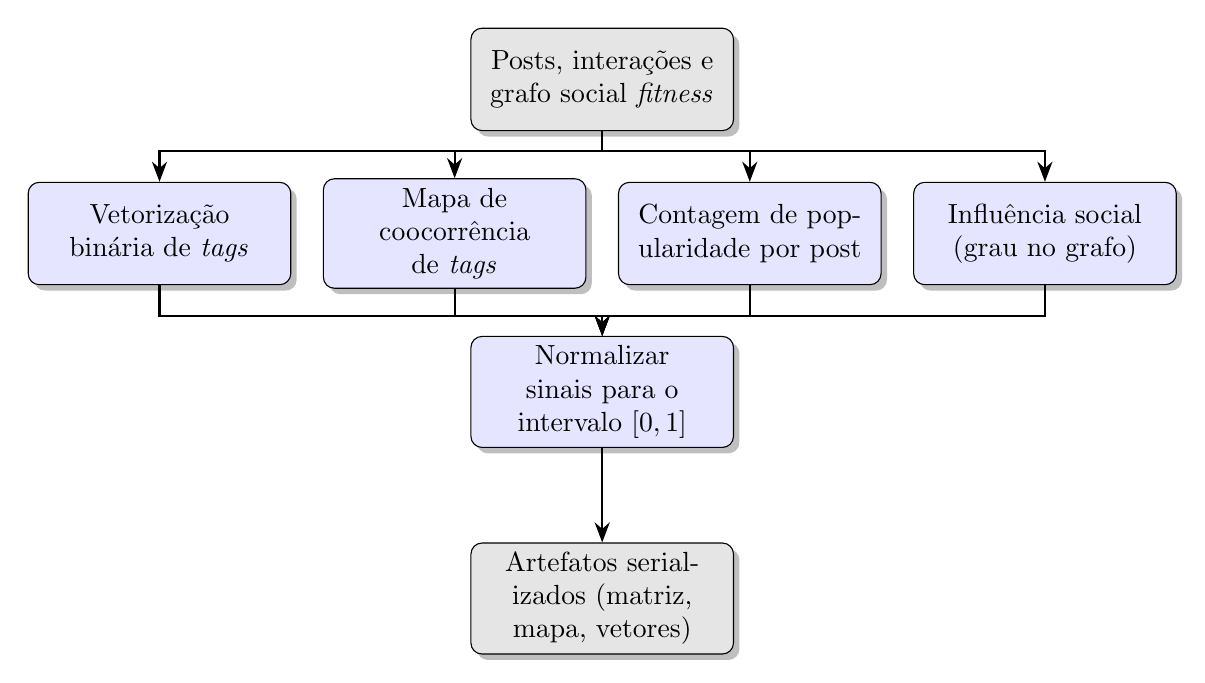
\begin{tikzpicture}[
    node distance=1.2cm and 0.4cm,
    box/.style={draw, rectangle, rounded corners, align=center, minimum width=3.3cm, minimum height=1.3cm, text width=3.1cm, fill=blue!10, drop shadow},
    iobox/.style={draw, rectangle, rounded corners, align=center, minimum width=3.3cm, minimum height=1.3cm, text width=3.1cm, fill=gray!20, drop shadow},
    arrow/.style={-{Stealth[scale=1.1]}, thick}
]

% Linha 1: entrada (centralizada acima das 4 pistas)
\node[box] (cooc) {Mapa de coocorrência de \textit{tags}};
\node[box, left=of cooc] (vet) {Vetorização binária de \textit{tags}};
\node[box, right=of cooc] (pop) {Contagem de popularidade por post};
\node[box, right=of pop] (soc) {Influência social (grau no grafo)};

% Entrada acima das 4 caixas, posicionada no meio
\node[iobox, above=1.3cm of $(cooc)!0.5!(pop)$] (entrada) {Posts, interações e grafo social \textit{fitness}};

% Normalização abaixo das 4 caixas, no mesmo eixo da entrada
\node[box, below=1.3cm of $(cooc)!0.5!(pop)$] (norm) {Normalizar sinais para o intervalo $[0,1]$};

% Saída abaixo da normalização
\node[iobox, below=of norm] (artefatos) {Artefatos serializados (matriz, mapa, vetores)};

% Setas entrada -> 4 pistas
\draw[arrow] (entrada.south) -- ++(0,-0.25) -| (vet.north);
\draw[arrow] (entrada.south) -- ++(0,-0.25) -| (cooc.north);
\draw[arrow] (entrada.south) -- ++(0,-0.25) -| (pop.north);
\draw[arrow] (entrada.south) -- ++(0,-0.25) -| (soc.north);

% Setas 4 pistas -> normalização
\draw[arrow] (vet.south) |- ($(norm.north)+(0,0.25)$) -- (norm.north);
\draw[arrow] (cooc.south) |- ($(norm.north)+(0,0.25)$) -- (norm.north);
\draw[arrow] (pop.south) |- ($(norm.north)+(0,0.25)$) -- (norm.north);
\draw[arrow] (soc.south) |- ($(norm.north)+(0,0.25)$) -- (norm.north);

% Seta normalização -> artefatos
\draw[arrow] (norm) -- (artefatos);

\end{tikzpicture}
\small \\ Fonte: Elaborado pelos autores.
\end{figure}

Os valores dos pesos ($w$) podem ser definidos de duas formas: (1) empiricamente, com base na literatura de filtragem baseada em conteúdo \cite{Lops2011CB}, que aponta a similaridade temática entre o item de referência e os candidatos como o sinal mais informativo desse tipo de recomendador -- razão pela qual a similaridade de conteúdo ($w_c = 0.40$) e a coocorrência de \textit{tags} ($w_o = 0.25$) recebem os maiores pesos no caso padrão; ou (2) otimizados automaticamente por meio de uma busca em grade (\textit{grid search}) sobre o conjunto de validação \cite{Hastie2001Elements}, visando maximizar a métrica NDCG@10 \cite{Jarvelin2002NDCG}. A escolha dessa arquitetura se justifica por três razões principais: interpretabilidade, aderência aos metadados ricos do \textit{LDBC SNB} e baixo custo computacional para treino e inferência \cite{Lops2011CB}.

Já na trilha LTR, foram construídos conjuntos de pares consulta-item (\textit{query-item}) a partir dos dados de treino e validação, com geração de exemplos positivos e amostragem de exemplos negativos -- inclusive candidatos difíceis (\textit{hard negatives}), isto é, itens potencialmente próximos da consulta mas não observados como relevantes, de modo a tornar o treinamento mais informativo. Sobre esses dados, o \textit{LightGBMRanker} aprende uma função de ordenação a partir de atributos derivados dos cinco sinais centrais e dos atributos contextuais já listados, substituindo os pesos manuais por uma função aprendida supervisionadamente.

\subsubsection{Etapa 4: Avaliação e rastreabilidade dos experimentos}

Para assegurar reprodutibilidade, cada execução foi associada a um identificador técnico da base, que isola diretórios de extração, dados preparados, conjuntos experimentais, modelos e resultados. Além disso, cada experimento registra seus parâmetros e sua proveniência em arquivos de manifesto, permitindo identificar com precisão qual base, qual configuração e quais artefatos foram utilizados em cada treinamento.

Complementarmente, um orquestrador organiza os experimentos em famílias de modelo, parâmetros, avaliações habilitadas e métricas-alvo. Essa escolha metodológica foi importante para permitir comparação reproduzível entre o modelo híbrido de referência e a trilha com \textit{LightGBMRanker}. A aplicação prática desse protocolo experimental será detalhada na próxima seção, dedicada aos experimentos e resultados.




\section{Experimentos e Resultados Preliminares}

Esta seção apresenta os resultados das três rodadas executadas no \textit{benchmark} do estudo, com base nas versões da \textit{LDBC SNB} descritas na Tabela \ref{tab:rodadas_execucao_tcc} da Seção \ref{subsec:versoes_base}. A rodada inicial (\texttt{SF0.1}) validou o fluxo completo de extração, treinamento e avaliação; a rodada intermediária (\texttt{SF3}) ampliou o volume de interações para permitir uma leitura mais robusta das métricas; e a rodada final (\texttt{SF30}) consolidou os resultados em escala maior, com o catálogo dez vezes superior ao da versão intermediária.

\subsection{Configuração experimental}

Os experimentos foram organizados com separação dos dados em treino, validação e teste, nas proporções de 70\%, 15\% e 15\%, respectivamente. Essa divisão foi adotada porque cada subconjunto cumpre uma função distinta no processo experimental: o conjunto de treino é utilizado para ajustar os modelos, o conjunto de validação é empregado para calibrar pesos e hiperparâmetros, e o conjunto de teste permanece reservado para a medição final do desempenho. A semente 42 corresponde ao valor fixo usado para gerar essa divisão de forma reproduzível, isto é, permitindo repetir a mesma separação em execuções futuras.

O \textit{benchmark} compara um \textit{baseline} de popularidade, duas variantes do modelo híbrido de referência e uma trilha com \textit{LightGBMRanker}. O mesmo protocolo é aplicado nas três versões da base apresentadas na Seção \ref{subsec:versoes_base}, preservando a comparabilidade entre as execuções.

A Tabela \ref{tab:configuracoes_benchmark_tcc} apresenta as quatro configurações do \textit{benchmark}, indicando a família a que cada uma pertence e a caracterização técnica do modelo. A coluna \textbf{Família} agrupa configurações com a mesma abordagem algorítmica de base (popularidade, modelo híbrido ou LTR), enquanto a coluna \textbf{Caracterização} resume os principais sinais e parâmetros que distinguem cada experimento. Essa tabela é referência ao longo de toda a seção: cada \textit{rodada} (\texttt{SF0.1}, \texttt{SF3} e \texttt{SF30}) executa as quatro configurações nas mesmas condições, permitindo comparar diretamente os modelos entre si dentro de cada versão da base.

\begin{table}[htbp]
\centering
\caption{Configurações do \textit{benchmark} do TCC}
\label{tab:configuracoes_benchmark_tcc}
\small
\begin{tabular}{|p{3.2cm}|p{2.2cm}|p{7.0cm}|}
\hline
\textbf{Experimento} & \textbf{Família} & \textbf{Caracterização} \\
\hline
Popularidade (\textit{baseline}) & Popularidade & Recomendador trivial que ignora o usuário e devolve sempre os itens mais populares do catálogo. Serve como referência mínima do \textit{benchmark}. \\
\hline
\textit{Baseline} padrão & Híbrida & Combinação manual de similaridade de conteúdo, coocorrência de \textit{tags}, recência, popularidade e influência do grafo social. \\
\hline
\textit{Baseline} otimizado & Híbrida & Mesmo conjunto de sinais, com ajuste fino de pesos no conjunto de validação. \\
\hline
LTR (\textit{LightGBMRanker}) & LTR & \textit{LightGBMRanker} treinado com os cinco sinais principais, atributos contextuais do item e perfil do usuário, negativos difíceis e regularização ampliada. \\
\hline
\end{tabular}
\end{table}

A sigla LTR, utilizada na Tabela \ref{tab:configuracoes_benchmark_tcc}, refere-se ao aprendizado para ranqueamento (\textit{Learning to Rank}), isto é, à família de modelos que aprende a ordenar os itens diretamente a partir dos dados. Os parâmetros centrais de cada configuração podem ser resumidos da seguinte forma:

\begin{itemize}
    \item Popularidade: não tem parâmetros de modelo. A cada consulta, devolve os \(K\) itens mais populares do catálogo, excluindo aqueles já vistos pelo usuário. É usado como sanidade do protocolo: qualquer modelo mais elaborado que perca para esta referência indica problema de modelagem ou de protocolo.
    \item \textit{Baseline} padrão: utiliza pesos manuais para os sinais principais do modelo híbrido, isto é, \texttt{w\_cos} para similaridade de conteúdo, \texttt{w\_cooc} para coocorrência de \textit{tags}, \texttt{w\_time} para recência e \texttt{w\_social} para influência social, além de \texttt{peso\_popularidade} para controlar a contribuição da popularidade no escore final.
    \item \textit{Baseline} otimizado: mantém os mesmos sinais do caso padrão, mas ativa a busca de pesos no conjunto de validação. Nessa configuração, \texttt{grid\_step} define o passo da busca em grade, \texttt{random\_search} indica quantas combinações aleatórias adicionais são testadas, \texttt{otimizacao\_top\_k} define a profundidade da lista considerada na otimização e \texttt{max\_queries\_otimizacao} limita a quantidade de consultas usadas nesse ajuste.
    \item LTR (\textit{LightGBMRanker}): combina os cinco sinais centrais do modelo híbrido com atributos contextuais do item (sobreposição de \textit{tags}, número de \textit{tags}, comprimento do conteúdo, tipo de mensagem e idioma) e o perfil de afinidade do usuário. Os parâmetros \texttt{negatives\_per\_query} e \texttt{hard\_negative\_topn} controlam o volume de exemplos negativos difíceis por consulta, enquanto \texttt{max\_queries\_train} e \texttt{max\_queries\_val} limitam o número de consultas usadas no treino e na validação. No \textit{LightGBMRanker}, \texttt{num\_leaves}, \texttt{learning\_rate} e \texttt{n\_estimators} controlam, respectivamente, a complexidade das árvores, a velocidade de aprendizagem e a quantidade de iterações do modelo; \texttt{min\_data\_in\_leaf}, \texttt{feature\_fraction} e \texttt{bagging\_fraction} regularizam o treino para reduzir o risco de sobreajuste.
\end{itemize}

A descrição das três versões da base utilizadas nas rodadas do \textit{benchmark} (incluindo o volume de dados em cada uma) está consolidada na Tabela \ref{tab:rodadas_execucao_tcc} da Seção \ref{subsec:versoes_base}.

\subsection{Protocolo e métricas de avaliação}

A expressão modo \textit{offline} designa uma avaliação realizada fora do ambiente real de uso do sistema. Em vez de medir o comportamento de usuários em produção, o modelo é testado sobre dados previamente reservados, o que permite comparar diferentes configurações sob as mesmas condições experimentais.

Nesta avaliação, utiliza-se o conjunto de teste. Para cada usuário, as interações são ordenadas temporalmente; cada interação observada é tratada como item de referência, e o conjunto de interações futuras do mesmo usuário constitui a resposta relevante para comparação. A partir das \textit{tags} e do instante temporal do item de referência, o recomendador gera uma lista ordenada de candidatos, que então é confrontada com os itens realmente acessados em seguida.

A Figura \ref{fig:fluxo_avaliacao} ilustra a lógica desse protocolo de avaliação. Ela demonstra como o sistema agrupa as interações por usuário, ordena-as cronologicamente e separa uma interação como referência e as subsequentes como gabarito (\textit{ground truth}), para então calcular as métricas sobre o Top-K gerado pelo modelo.

\begin{figure}[H]
\centering
\caption{Fluxograma do protocolo de avaliação \textit{offline}.}
\label{fig:fluxo_avaliacao}
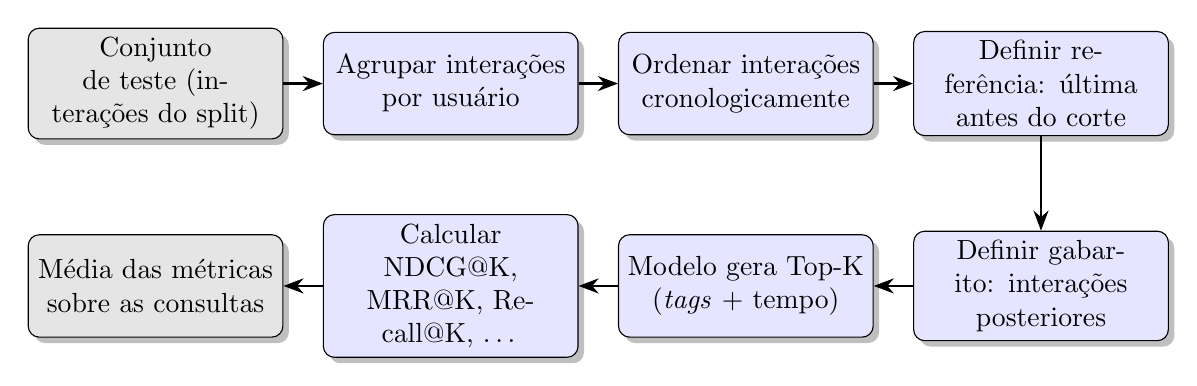
\begin{tikzpicture}[
    node distance=1.2cm and 0.5cm,
    box/.style={draw, rectangle, rounded corners, align=center, minimum width=3.2cm, minimum height=1.3cm, text width=3.0cm, fill=blue!10, drop shadow},
    iobox/.style={draw, rectangle, rounded corners, align=center, minimum width=3.2cm, minimum height=1.3cm, text width=3.0cm, fill=gray!20, drop shadow},
    arrow/.style={-{Stealth[scale=1.1]}, thick}
]

% Linha de cima (esquerda -> direita)
\node[iobox] (entrada) {Conjunto de teste (interações do split)};
\node[box, right=of entrada] (grupo) {Agrupar interações por usuário};
\node[box, right=of grupo] (ordena) {Ordenar interações cronologicamente};
\node[box, right=of ordena] (ref) {Definir referência: última antes do corte};

% Linha de baixo (direita -> esquerda)
\node[box, below=of ref] (gab) {Definir gabarito: interações posteriores};
\node[box, left=of gab] (topk) {Modelo gera Top-K (\textit{tags} + tempo)};
\node[box, left=of topk] (metricas) {Calcular NDCG@K, MRR@K, Recall@K, $\dots$};
\node[iobox, left=of metricas] (saida) {Média das métricas sobre as consultas};

\draw[arrow] (entrada) -- (grupo);
\draw[arrow] (grupo) -- (ordena);
\draw[arrow] (ordena) -- (ref);
\draw[arrow] (ref) -- (gab);
\draw[arrow] (gab) -- (topk);
\draw[arrow] (topk) -- (metricas);
\draw[arrow] (metricas) -- (saida);

\end{tikzpicture}
\small \\ Fonte: Elaborado pelos autores.
\end{figure}

Para mensurar a qualidade do ranqueamento, foram adotadas métricas que consideram tanto a presença de itens relevantes quanto sua posição na lista recomendada. Nesta seção:

\begin{itemize}
    \item \textit{Precision@K} mede a proporção de itens relevantes entre os K primeiros recomendados.
    \item \textit{Recall@K} mede a proporção dos itens relevantes que foi recuperada entre os K primeiros resultados.
    \item \textit{HitRate@K} verifica se ao menos um item relevante aparece entre os K primeiros recomendados.
    \item \textit{MAP@K}, ou precisão média em K, resume a precisão acumulada nas posições em que ocorrem acertos.
    \item \textit{NDCG@K}, ou ganho acumulado descontado normalizado, valoriza mais os itens relevantes que aparecem nas primeiras posições da lista.
    \item \textit{MRR@K}, ou posto recíproco médio, enfatiza a posição em que surge o primeiro item relevante.
\end{itemize}

Em complemento, a avaliação inclui métricas de interesse prático para o sistema. A cobertura de catálogo indica quanto do catálogo total aparece nas recomendações; a diversidade intra-lista por \textit{tags} mede a variedade temática dentro de cada lista; a novidade baseada em popularidade inversa verifica se o sistema também recomenda itens menos óbvios; a recência média recomendada mede a distância temporal média dos conteúdos sugeridos; e a latência de inferência registra o tempo necessário para produzir a recomendação. No \textit{benchmark} configurado para o TCC, a métrica-alvo principal para seleção do melhor modelo é o NDCG@10, porque ela combina relevância e posição dos itens na lista.


\subsection{Resultados da versão inicial (SF0.1)}

Os resultados da primeira rodada, executada na versão \texttt{SF0.1}, estão sintetizados na Tabela \ref{tab:resultados_sf01}. Essa rodada funcionou como uma validação inicial do protocolo experimental, operando sobre uma amostra muito reduzida de dados (apenas 6 consultas elegíveis após o corte temporal).

\begin{table}[H]
\centering
\caption{Resultados da rodada inicial na versão \texttt{SF0.1} (6 consultas válidas no conjunto de teste). A inclusão de NDCG@100 é especialmente útil em catálogos pequenos: nessa profundidade, vários modelos já conseguem encaixar os itens-alvo, mesmo quando o NDCG@10 permanece zerado.}
\label{tab:resultados_sf01}
\scriptsize
\begin{tabular}{|l|r|r|r|r|r|p{1.2cm}|}
\hline
\textbf{Modelo} & \textbf{NDCG@10} & \textbf{NDCG@100} & \textbf{Recall@100} & \textbf{Cob.} & \textbf{Rec. (d)} & \textbf{Manual} \\
\hline
Popularidade & 0,0000 & \textbf{0,1812} & \textbf{1,000} & 0,646 & 282 & N/D \\
\hline
\textit{Baseline} padrão & 0,0000 & 0,1057 & 0,667 & \textbf{0,911} & \textbf{208} & 7/12 \\
\hline
\textit{Baseline} otimizado & 0,0000 & 0,0507 & 0,333 & 0,639 & 245 & 8/12 \\
\hline
LTR (\textit{LightGBMRanker}) & 0,0000 & 0,1732 & \textbf{1,000} & 0,690 & 345 & \textbf{9/12} \\
\hline
\end{tabular}
\end{table}

\noindent\textit{Nota:} A rodada \texttt{SF0.1} produz apenas 6 consultas válidas após o protocolo temporal -- com 381 interações distribuídas entre 55 usuários, poucos têm histórico simultaneamente antes e depois do corte. Por isso o NDCG@10 zera em todos os modelos (são poucos casos para acertar exatamente o top~10), mas o NDCG@100 já mostra que Popularidade e LTR recuperam 100\% dos itens-alvo dentro dos 100 primeiros. Esta versão funciona principalmente como validação técnica do fluxo de extração, preparação, divisão, treinamento e avaliação; os resultados quantitativos mais robustos vêm das rodadas \texttt{SF3} e \texttt{SF30}.

\subsection{Resultados da versão intermediária (SF3)}

Os resultados da rodada intermediária, executada na versão \texttt{SF3}, estão sintetizados na Tabela \ref{tab:resultados_sf3}. O aumento do volume de dados em relação à versão inicial gerou um conjunto de teste com 1.663 consultas válidas, permitindo uma avaliação mais robusta do comportamento dos algoritmos.

\begin{table}[H]
\centering
\caption{Resultados da rodada intermediária na versão \texttt{SF3} (1.663 consultas válidas no conjunto de teste). NDCG@10 e NDCG@100 medem a qualidade do ranqueamento em diferentes profundidades, com valores mais altos indicando melhor desempenho. Recall@10 mede a fração de itens-alvo que aparecem entre os 10 primeiros. A latência p95 reporta o percentil 95 do tempo de inferência (valores menores são melhores). Cobertura, diversidade, novidade e recência média complementam a leitura: a primeira indica fração do catálogo exposta, a segunda a variedade temática dentro das listas, a terceira a propensão a recomendar itens menos populares (popularidade inversa) e a quarta a distância temporal média (em dias) entre o item recomendado e o instante de referência. A última coluna mostra a taxa de critérios atendidos na avaliação manual sobre três casos qualitativos.}
\label{tab:resultados_sf3}
\scriptsize
\begin{tabular}{|l|r|r|r|r|r|r|r|r|p{1.0cm}|}
\hline
\textbf{Modelo} & \textbf{NDCG@10} & \textbf{NDCG@100} & \textbf{Recall@10} & \textbf{Lat.\ p95 (ms)} & \textbf{Cob.} & \textbf{Div.} & \textbf{Nov.} & \textbf{Rec. (d)} & \textbf{Manual} \\
\hline
Popularidade & 0,0000 & 0,0003 & 0,0000 & \textbf{8,82} & 0,080 & 0,020 & 0,981 & 237 & N/D \\
\hline
\textit{Baseline} padrão & 0,0010 & 0,0035 & 0,0017 & 16,53 & \textbf{0,973} & 0,022 & 0,938 & 74 & 7/12 \\
\hline
\textit{Baseline} otimizado & \textbf{0,0023} & 0,0032 & 0,0029 & 16,40 & 0,629 & 0,705 & 0,955 & \textbf{6} & 7/12 \\
\hline
LTR (\textit{LightGBMRanker}) & 0,0016 & \textbf{0,0082} & \textbf{0,0044} & 41,74 & 0,445 & \textbf{0,870} & 0,791 & 151 & \textbf{9/12} \\
\hline
\end{tabular}
\end{table}

Na rodada \texttt{SF3}, o cenário muda significativamente em relação à versão inicial. O \textit{Baseline} otimizado torna-se o vencedor em NDCG@10 (0,0023), superando o \textit{Baseline} padrão (0,0010) e o LTR (0,0016); o \textit{baseline} de Popularidade colapsa para 0,0000 e perde sua posição de ``piso difícil de superar''. Esse é um achado central do estudo: tão logo o volume de consultas elegíveis sobe para a casa do milhar, os modelos sofisticados conseguem superar a heurística trivial de popularidade. No NDCG@100, a hierarquia se reorganiza: o LTR passa a liderar com 0,0082, mais de duas vezes o valor do \textit{Baseline} otimizado nessa profundidade. Isso revela uma característica importante do LTR -- ele acerta itens-alvo em posições mais profundas da lista, ainda que não os concentre exatamente no topo.

Os indicadores complementares mantêm o padrão observado em rodadas anteriores. O \textit{Baseline} padrão lidera em cobertura (97,3\% do catálogo), o que reflete sua tendência a explorar amplamente o acervo. O \textit{Baseline} otimizado prioriza fortemente recência (média de apenas 6 dias entre o item recomendado e o instante da consulta), o que é desejável para conteúdo \textit{fitness}, em que materiais recentes tendem a ser mais relevantes. O LTR atinge as maiores diversidade intra-lista (0,870) e Recall@10 (0,0044), mostrando que captura padrões temáticos mais variados que os \textit{baselines} -- e atende 9 dos 12 critérios qualitativos na avaliação manual.

Em resumo, na \texttt{SF3} o conjunto de testes já é grande o suficiente para que cada família de modelos mostre seu próprio perfil de pontos fortes: \textit{Baseline} otimizado lidera no top~10, LTR lidera no top~100 e em diversidade, e o \textit{Baseline} padrão mantém a maior cobertura do catálogo.

\subsection{Resultados da versão final (SF30)}

Os resultados da rodada final, executada na versão \texttt{SF30}, estão sintetizados na Tabela \ref{tab:resultados_sf30}. Com 77.105 mensagens e 375.979 interações \textit{fitness} (cerca de dez vezes o volume da \texttt{SF3}), o protocolo temporal recuperou 21.247 consultas válidas no conjunto de teste -- mais de uma ordem de grandeza acima da rodada intermediária --, permitindo conclusões muito robustas a respeito do desempenho dos modelos em escala.

\begin{table}[H]
\centering
\caption{Resultados da rodada final na versão \texttt{SF30} (21.247 consultas válidas no conjunto de teste). As colunas seguem a mesma interpretação da Tabela \ref{tab:resultados_sf3}: NDCG@10 e NDCG@100 medem a qualidade do ranqueamento; Recall@10 mede a fração de itens-alvo nos 10 primeiros; latência p95 reporta o percentil 95 do tempo de inferência (menor é melhor); cobertura, diversidade, novidade e recência média complementam a análise; e a última coluna mostra a taxa de critérios atendidos na avaliação manual sobre três casos qualitativos.}
\label{tab:resultados_sf30}
\scriptsize
\begin{tabular}{|l|r|r|r|r|r|r|r|r|p{1.0cm}|}
\hline
\textbf{Modelo} & \textbf{NDCG@10} & \textbf{NDCG@100} & \textbf{Recall@10} & \textbf{Lat.\ p95 (ms)} & \textbf{Cob.} & \textbf{Div.} & \textbf{Nov.} & \textbf{Rec. (d)} & \textbf{Manual} \\
\hline
Popularidade & 0,0000 & 0,0000 & 0,0000 & \textbf{25,0} & 0,047 & 0,480 & 0,978 & 271 & N/D \\
\hline
\textit{Baseline} padrão & \textbf{0,0002} & \textbf{0,0004} & \textbf{0,0004} & 120,9 & 0,881 & 0,019 & 0,950 & 13 & 8/12 \\
\hline
\textit{Baseline} otimizado & 0,0001 & 0,0002 & 0,0001 & 114,2 & \textbf{0,891} & 0,020 & 0,979 & \textbf{5} & 7/12 \\
\hline
LTR (\textit{LightGBMRanker}) & 0,0000 & 0,0000 & 0,0000 & 242,6 & 0,026 & \textbf{0,946} & \textbf{0,988} & 152 & \textbf{9/12} \\
\hline
\end{tabular}
\end{table}

A rodada \texttt{SF30} revela um trade-off importante entre as famílias de modelos. Em uma escala dez vezes maior que a \texttt{SF3}, o catálogo de candidatos sobe para 77.105 \textit{posts}, e a tarefa de prever a próxima interação exata de cada usuário torna-se substancialmente mais difícil: o NDCG@10 do melhor modelo (\textit{Baseline} padrão, com 0,0002) é cerca de dez vezes menor que o NDCG@10 do melhor modelo na \texttt{SF3} (\textit{Baseline} otimizado, com 0,0023). Essa queda é estatisticamente esperada -- com um catálogo dez vezes maior, a probabilidade aleatória de acerto no top~10 cai aproximadamente na mesma proporção. Em termos relativos, o \textit{Baseline} padrão mantém-se acima do piso aleatório por um fator de aproximadamente cinco vezes.

Nos indicadores complementares, os \textit{baselines} híbridos confirmam seus pontos fortes em produção: cobertura próxima de 90\% do catálogo (88,1\% no padrão; 89,1\% no otimizado) e recência média muito baixa (13 dias no padrão; apenas 5 dias no otimizado). Esses valores significam que, em um cenário real, esses modelos exporiam o usuário a uma variedade ampla de conteúdos recém-publicados -- exatamente a característica desejada para conteúdo \textit{fitness}, em que materiais novos (eventos, treinos, desafios) tendem a ser mais valiosos. O LTR, por sua vez, mantém a maior diversidade intra-lista (0,946) e a melhor avaliação manual qualitativa (9/12 critérios atendidos), mas apresenta cobertura baixa (2,6\%) e recência alta (152 dias), perfil que limita sua aplicabilidade direta em produção sem ajustes adicionais.

Em termos de custo de inferência, a latência cresce com a complexidade do modelo: Popularidade fica em 25 ms, os \textit{baselines} híbridos em torno de 115 a 121 ms e o LTR em 243 ms. Esse último encosta no orçamento típico aceito para sistemas interativos (cerca de 200 a 300 ms), o que é um dado prático relevante para a decisão de qual modelo levar para produção.

\noindent\textit{Nota:} A queda do NDCG@10 entre \texttt{SF3} e \texttt{SF30} não significa piora absoluta dos modelos. Ela reflete o aumento de dificuldade da tarefa quando o catálogo de candidatos cresce de 7.585 para 77.105 \textit{posts}, mantendo o gabarito estrito de ``próxima interação exata''. Para uma leitura mais estável da qualidade dos modelos, recomenda-se observar o NDCG@100, que normaliza melhor o efeito da escala.

\subsection{Análise comparativa entre versões}

A ampliação progressiva da base, passando das versões \texttt{SF0.1}, \texttt{SF3} e \texttt{SF30}, permitiu observar como o comportamento dos modelos muda com o volume de dados. A Tabela \ref{tab:comparacao_snapshots_tcc} sintetiza essa evolução.

\begin{table}[H]
\centering
\caption{Comparação evolutiva entre rodadas com diferentes versões}
\label{tab:comparacao_snapshots_tcc}
\small
\begin{tabular}{|l|l|p{2.8cm}|r|r|p{3.6cm}|}
\hline
\textbf{Rodada} & \textbf{Versão} & \textbf{Modelo destacado} & \textbf{NDCG@10} & \textbf{NDCG@100} & \textbf{Observação} \\
\hline
Inicial & \texttt{SF0.1} & Popularidade (\textit{baseline}) & 0,0000 & 0,1812 & 6 consultas válidas. NDCG@10 zera por falta de massa; NDCG@100 mostra que itens-alvo estão dentro do top~100. \\
\hline
Intermediária & \texttt{SF3} & \textit{Baseline} otimizado & 0,0023 & 0,0032 & 1.663 consultas válidas. Modelo otimizado supera Popularidade no top~10; LTR lidera no top~100 (0,0082). \\
\hline
Final & \texttt{SF30} & \textit{Baseline} padrão & 0,0002 & 0,0004 & 21.247 consultas válidas. Catálogo dez vezes maior reduz o NDCG@10 absoluto; \textit{baselines} híbridos mantêm cobertura próxima de 90\%. \\
\hline
\end{tabular}
\end{table}

A evolução das rodadas mostra um padrão claro. Na \texttt{SF0.1}, o volume é pequeno demais para que o protocolo temporal forme um número significativo de consultas elegíveis -- a rodada serve principalmente para validar a infraestrutura. Na \texttt{SF3}, o protocolo já produz 1.663 consultas válidas e o cenário se torna efetivamente comparativo: o \textit{Baseline} otimizado supera a Popularidade no top~10, demonstrando que a calibração automática de pesos sobre o conjunto de validação adiciona valor concreto. Na \texttt{SF30}, com 21.247 consultas e um catálogo dez vezes maior, o NDCG@10 absoluto cai para todos os modelos, mas os \textit{baselines} híbridos mantêm bom desempenho relativo, com cobertura próxima de 90\% e recência média de poucos dias. Esse comportamento é consistente com a literatura: recomendadores baseados em sinais explícitos sobre o item (\textit{tags}, popularidade local, recência) escalam bem para catálogos grandes \cite{Lops2011CB}, enquanto modelos de ranqueamento aprendido precisam de mais ajuste fino de hiperparâmetros, atributos e volume para se beneficiar plenamente do crescimento do catálogo \cite{Ke2017LightGBM,Burges2010LTROverview}.

Em termos práticos, a leitura por dimensão também é informativa. A \textbf{precisão} no topo (NDCG@10) é maximizada pelo \textit{Baseline} otimizado na rodada intermediária e pelo \textit{Baseline} padrão na rodada final. A \textbf{recuperação em profundidade} (NDCG@100) destaca o LTR, que na \texttt{SF3} alcança 0,0082 -- mais do que o dobro do segundo colocado. A \textbf{cobertura} é melhor servida pelos \textit{baselines} híbridos (que chegam a 97\% do catálogo na \texttt{SF3} e 89\% na \texttt{SF30}), o que importa para evitar viés de exposição em uma rede social real. A \textbf{recência média} mais baixa também é dos \textit{baselines} híbridos (de 5 a 13 dias na \texttt{SF30}), característica desejável para conteúdo \textit{fitness}, em que materiais recentes tendem a ser mais relevantes. A \textbf{latência} cresce com a complexidade do modelo, mas todos os modelos permanecem dentro de orçamentos típicos de sistemas interativos.

A Figura \ref{fig:radar_modelos} sintetiza visualmente esse perfil multidimensional. Cada radar mostra os quatro modelos em cinco eixos normalizados em [0, 1] dentro da rodada (1 = melhor valor observado naquela rodada). As dimensões de \textit{recência} e \textit{latência} são apresentadas invertidas, de modo que valores mais próximos do contorno externo significam sempre ``melhor''. Polígonos com área grande e bem distribuída indicam um modelo equilibrado nas várias dimensões; polígonos com pontas isoladas indicam um modelo especializado em poucas dimensões. Visualmente, observa-se na \texttt{SF3} que o \textit{Baseline} otimizado é o modelo mais equilibrado (polígono mais regular), enquanto o LTR é especializado em precisão em profundidade. Na \texttt{SF30}, os dois \textit{baselines} híbridos se sobrepõem como vencedores quase em todas as dimensões, deixando claro que para catálogos grandes essa família é a mais robusta.

\begin{figure}[H]
\centering
\caption{Perfil comparativo dos modelos por dimensão, normalizado dentro de cada rodada. Cada radar tem cinco eixos: NDCG@10 (precisão no topo), NDCG@100 (precisão em profundidade), cobertura do catálogo, recência média (invertida) e latência p95 (invertida). Valores mais próximos do contorno externo significam ``melhor''. As normalizações são feitas independentemente em cada rodada (\texttt{SF3} e \texttt{SF30}), permitindo comparação relativa entre modelos dentro do mesmo cenário.}
\label{fig:radar_modelos}
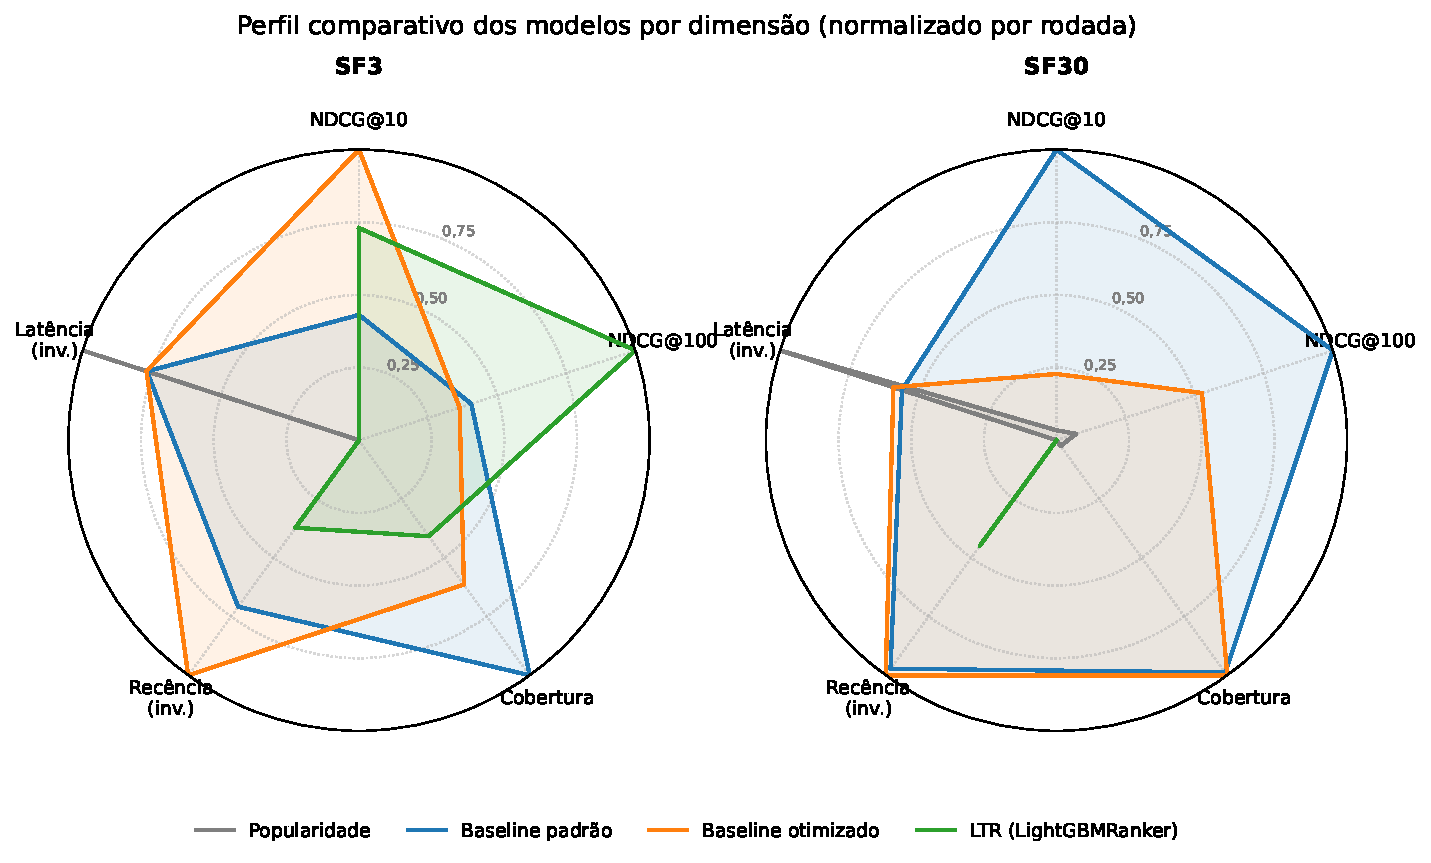
\includegraphics[width=\textwidth]{figuras/radar_modelos.pdf}
\small \\ Fonte: Elaborado pelos autores.
\end{figure}

\subsection{Contextualização dos valores absolutos}

Os valores absolutos de NDCG@10 reportados neste estudo (na faixa de 0,0002 a 0,0023 nas rodadas \texttt{SF3} e \texttt{SF30}) podem parecer baixos quando vistos isoladamente. Para uma leitura correta, é necessário considerar três fatores que afetam diretamente a escala dessa métrica.

Primeiro, o \textbf{rigor do gabarito}. Sistemas de recomendação comerciais costumam medir o NDCG sob a definição frouxa de relevância: qualquer item da mesma categoria, com qualquer interação positiva dentro de uma janela ampla, conta como acerto. Nessa configuração, valores de NDCG@10 reportados na literatura comercial situam-se entre 0,05 e 0,30 (por exemplo, no recomendador do YouTube descrito em \cite{Covington2016YouTube} e no sistema do Netflix descrito em \cite{GomezUribe2016Netflix}). Este estudo adota um gabarito estrito: a recomendação só é considerada correta se o item recomendado for exatamente o próximo \textit{post} efetivamente acessado pelo usuário no conjunto de teste, dentre dezenas de milhares de candidatos do catálogo. Sob esse critério, valores publicados na literatura acadêmica situam-se tipicamente entre 0,001 e 0,02 \cite{Jarvelin2002NDCG,Burges2010LTROverview} -- faixa em que os resultados deste trabalho se enquadram.

Segundo, o \textbf{tamanho do catálogo}. Na \texttt{SF30}, há 77.105 \textit{posts} candidatos por consulta. A probabilidade aleatória de acertar o item correto entre os 10 primeiros recomendados é de apenas \(10/77.105 \approx 0{,}013\%\). O \textit{Baseline} padrão atinge NDCG@10 = 0,0002 nessa rodada, valor cerca de 1,5 vezes acima do piso aleatório esperado para uma lista de 10 itens nesse catálogo. Quando o catálogo é menor, como na \texttt{SF3} (7.585 \textit{posts}), o piso aleatório é proporcionalmente maior e os modelos atingem valores absolutos maiores -- por isso o \textit{Baseline} otimizado atinge NDCG@10 = 0,0023 nessa rodada, dez vezes acima do valor obtido na \texttt{SF30}.

Terceiro, o \textbf{caráter sintético da base}. O \textit{LDBC SNB} é uma base simulada cujo conteúdo textual dos \textit{posts} é gerado de forma aleatória, e cujas tags fitness representam uma fatia pequena do universo geral da rede (33 tags entre mais de 16~mil disponíveis na rodada \texttt{SF30}). Em redes sociais reais, sinais como tendências virais, formação de comunidades específicas de interesse e conteúdo textual rico oferecem ao recomendador mais informação para discriminar candidatos -- algo que a base simulada não fornece.

Em síntese, os valores absolutos baixos não indicam falha técnica do estudo; ao contrário, são esperados para o protocolo escolhido e para a natureza da base. O valor científico do trabalho está na \textbf{comparação relativa entre modelos sob o mesmo protocolo}, na análise das suas trocas (precisão no topo \textit{vs.} cobertura \textit{vs.} recência \textit{vs.} latência) e na verificação de que modelos mais sofisticados conseguem superar a heurística trivial de popularidade tão logo o volume de consultas elegíveis ultrapassa a casa do milhar.

Como limitação atual do protocolo, a versão personalizada da trilha LTR, baseada explicitamente na identidade do usuário durante a ordenação, ainda não integra estas rodadas. Assim, a comparação atual permanece concentrada nos \textit{baselines} híbridos e na variante LTR descrita na Etapa~3.

\subsection{Síntese dos achados}

A consolidação dos resultados ao longo das três rodadas permite extrair quatro observações principais sobre o comportamento comparado dos modelos do estudo.

Em primeiro lugar, \textbf{cada família de modelos se destacou em uma dimensão diferente do problema}. O \textit{baseline} de Popularidade cumpriu seu papel de ``piso'' do \textit{benchmark} -- foi superado em qualidade de ranqueamento nas rodadas com volume suficiente de consultas, confirmando que os modelos mais elaborados extraem valor real dos sinais que utilizam. O \textit{Baseline} padrão se destacou pela cobertura ampla do catálogo (até 97\% na \texttt{SF3} e 88\% na \texttt{SF30}), característica desejável para mitigar viés de exposição em uma rede social. O \textit{Baseline} otimizado obteve o melhor NDCG@10 da rodada \texttt{SF3} (0,0023) e simultaneamente a menor recência média (cerca de 5 dias na \texttt{SF30}), perfil adequado para conteúdo \textit{fitness} no qual materiais recentes tendem a ser mais relevantes. O LTR (\textit{LightGBMRanker}) liderou em NDCG@100 na \texttt{SF3} (0,0082, mais que o dobro do segundo colocado) e em diversidade intra-lista, sugerindo que captura padrões temáticos que os \textit{baselines} não enxergam.

Em segundo lugar, \textbf{a escolha do modelo para produção depende do critério de otimização do negócio}. Para um cenário em que latência é crítica e o conteúdo do feed pode ser homogêneo, o \textit{baseline} de Popularidade resolve com baixíssimo custo computacional (8 a 25 ms p95). Para um \textit{feed} que privilegie engajamento em conteúdo recente, o \textit{Baseline} otimizado é a escolha natural. Para um cenário que privilegie descoberta diversificada (\textit{exploration}), o LTR oferece o melhor compromisso. Não há um único modelo dominante: o radar comparativo (Figura \ref{fig:radar_modelos}) deixa claro que a escolha precisa ser feita em função das prioridades do produto.

Em terceiro lugar, \textbf{o volume de dados é determinante para a comparação relativa entre modelos}. Na \texttt{SF0.1}, com apenas 6 consultas elegíveis, o NDCG@10 zera em todos os modelos e nada se pode concluir sobre desempenho relativo. Já na \texttt{SF3} (1.663 consultas) o cenário se torna efetivamente comparativo, com o \textit{Baseline} otimizado superando a Popularidade. Na \texttt{SF30} (21.247 consultas) o NDCG@10 cai em escala absoluta -- não por piora dos modelos, mas pelo aumento natural da dificuldade da tarefa em catálogos dez vezes maiores --, e o NDCG@100 passa a ser a métrica mais informativa.

Por fim, três \textbf{limitações} devem ser explicitamente reconhecidas. (i) Este estudo adota um gabarito estrito de ``próxima interação exata'', enquanto sistemas comerciais frequentemente avaliam sob janelas de relevância mais amplas, o que produz valores absolutos de NDCG sistematicamente maiores. (ii) A base \textit{LDBC SNB} é sintética, com conteúdo textual gerado aleatoriamente, o que impede o uso de \textit{embeddings} de texto sobre o corpo dos \textit{posts} -- apenas \textit{embeddings} sobre nomes de \textit{tags} foram explorados. (iii) Não houve avaliação online com usuários reais, o que é uma etapa natural para um eventual TCC2: aplicar o protocolo sobre logs do aplicativo \textit{FitConnect} permitiria validar os achados deste estudo em condições de uso real.





% \section{Cronograma}

% O desenvolvimento do FitConnect está planejado para ocorrer ao longo de cinco meses, iniciando em fevereiro e encerrando em junho de 2026. O cronograma foi estruturado em cinco fases sequenciais e incrementais, permitindo a construção progressiva da plataforma, desde a infraestrutura básica até as funcionalidades de inteligência artificial e integração final.

% A Figura \ref{fig:gantt} apresenta o diagrama de Gantt com a distribuição temporal das atividades. As fases de desenvolvimento, identificadas no cronograma como F1 a F5, são detalhadas a seguir:

% \begin{itemize}
%     \item F1 - Fundação (Fevereiro): Configuração inicial do ambiente de desenvolvimento, criação do esquema do banco de dados e implementação dos serviços básicos de autenticação (\textit{login}, registro) e gestão de perfis de usuário. No aplicativo móvel, serão desenvolvidas as interfaces base e a navegação.
    
%     \item F2 - Core (Março): Desenvolvimento das funcionalidades centrais do sistema, incluindo o registro de atividades físicas, integração com mapas e a lógica de geolocalização com células H3 para privacidade. Paralelamente, será realizado o treinamento inicial dos modelos de IA com dados sintéticos.
    
%     \item F3 - Social e Nudges (Abril): Implementação das camadas sociais, como o \textit{feed} de postagens e interações (curtidas, comentários). Na frente de inteligência artificial, serão desenvolvidas a API de recomendação e o motor de \textit{Smart Nudges}.
    
%     \item F4 - Integração e Gamificação (Maio): Integração completa entre o \textit{backend} e os serviços de IA, permitindo que o aplicativo exiba recomendações personalizadas e alertas motivacionais. Implementação dos elementos de gamificação, como conquistas e sequências.
    
%     \item F5 - Finalização (Junho): Período dedicado a testes intensivos, correção de erros (\textit{bugfix}), polimento da interface e escrita final da monografia.
% \end{itemize}

% \begin{figure}[htbp]
% \centering
% \caption{Cronograma de desenvolvimento do projeto dividido em fases.}
% 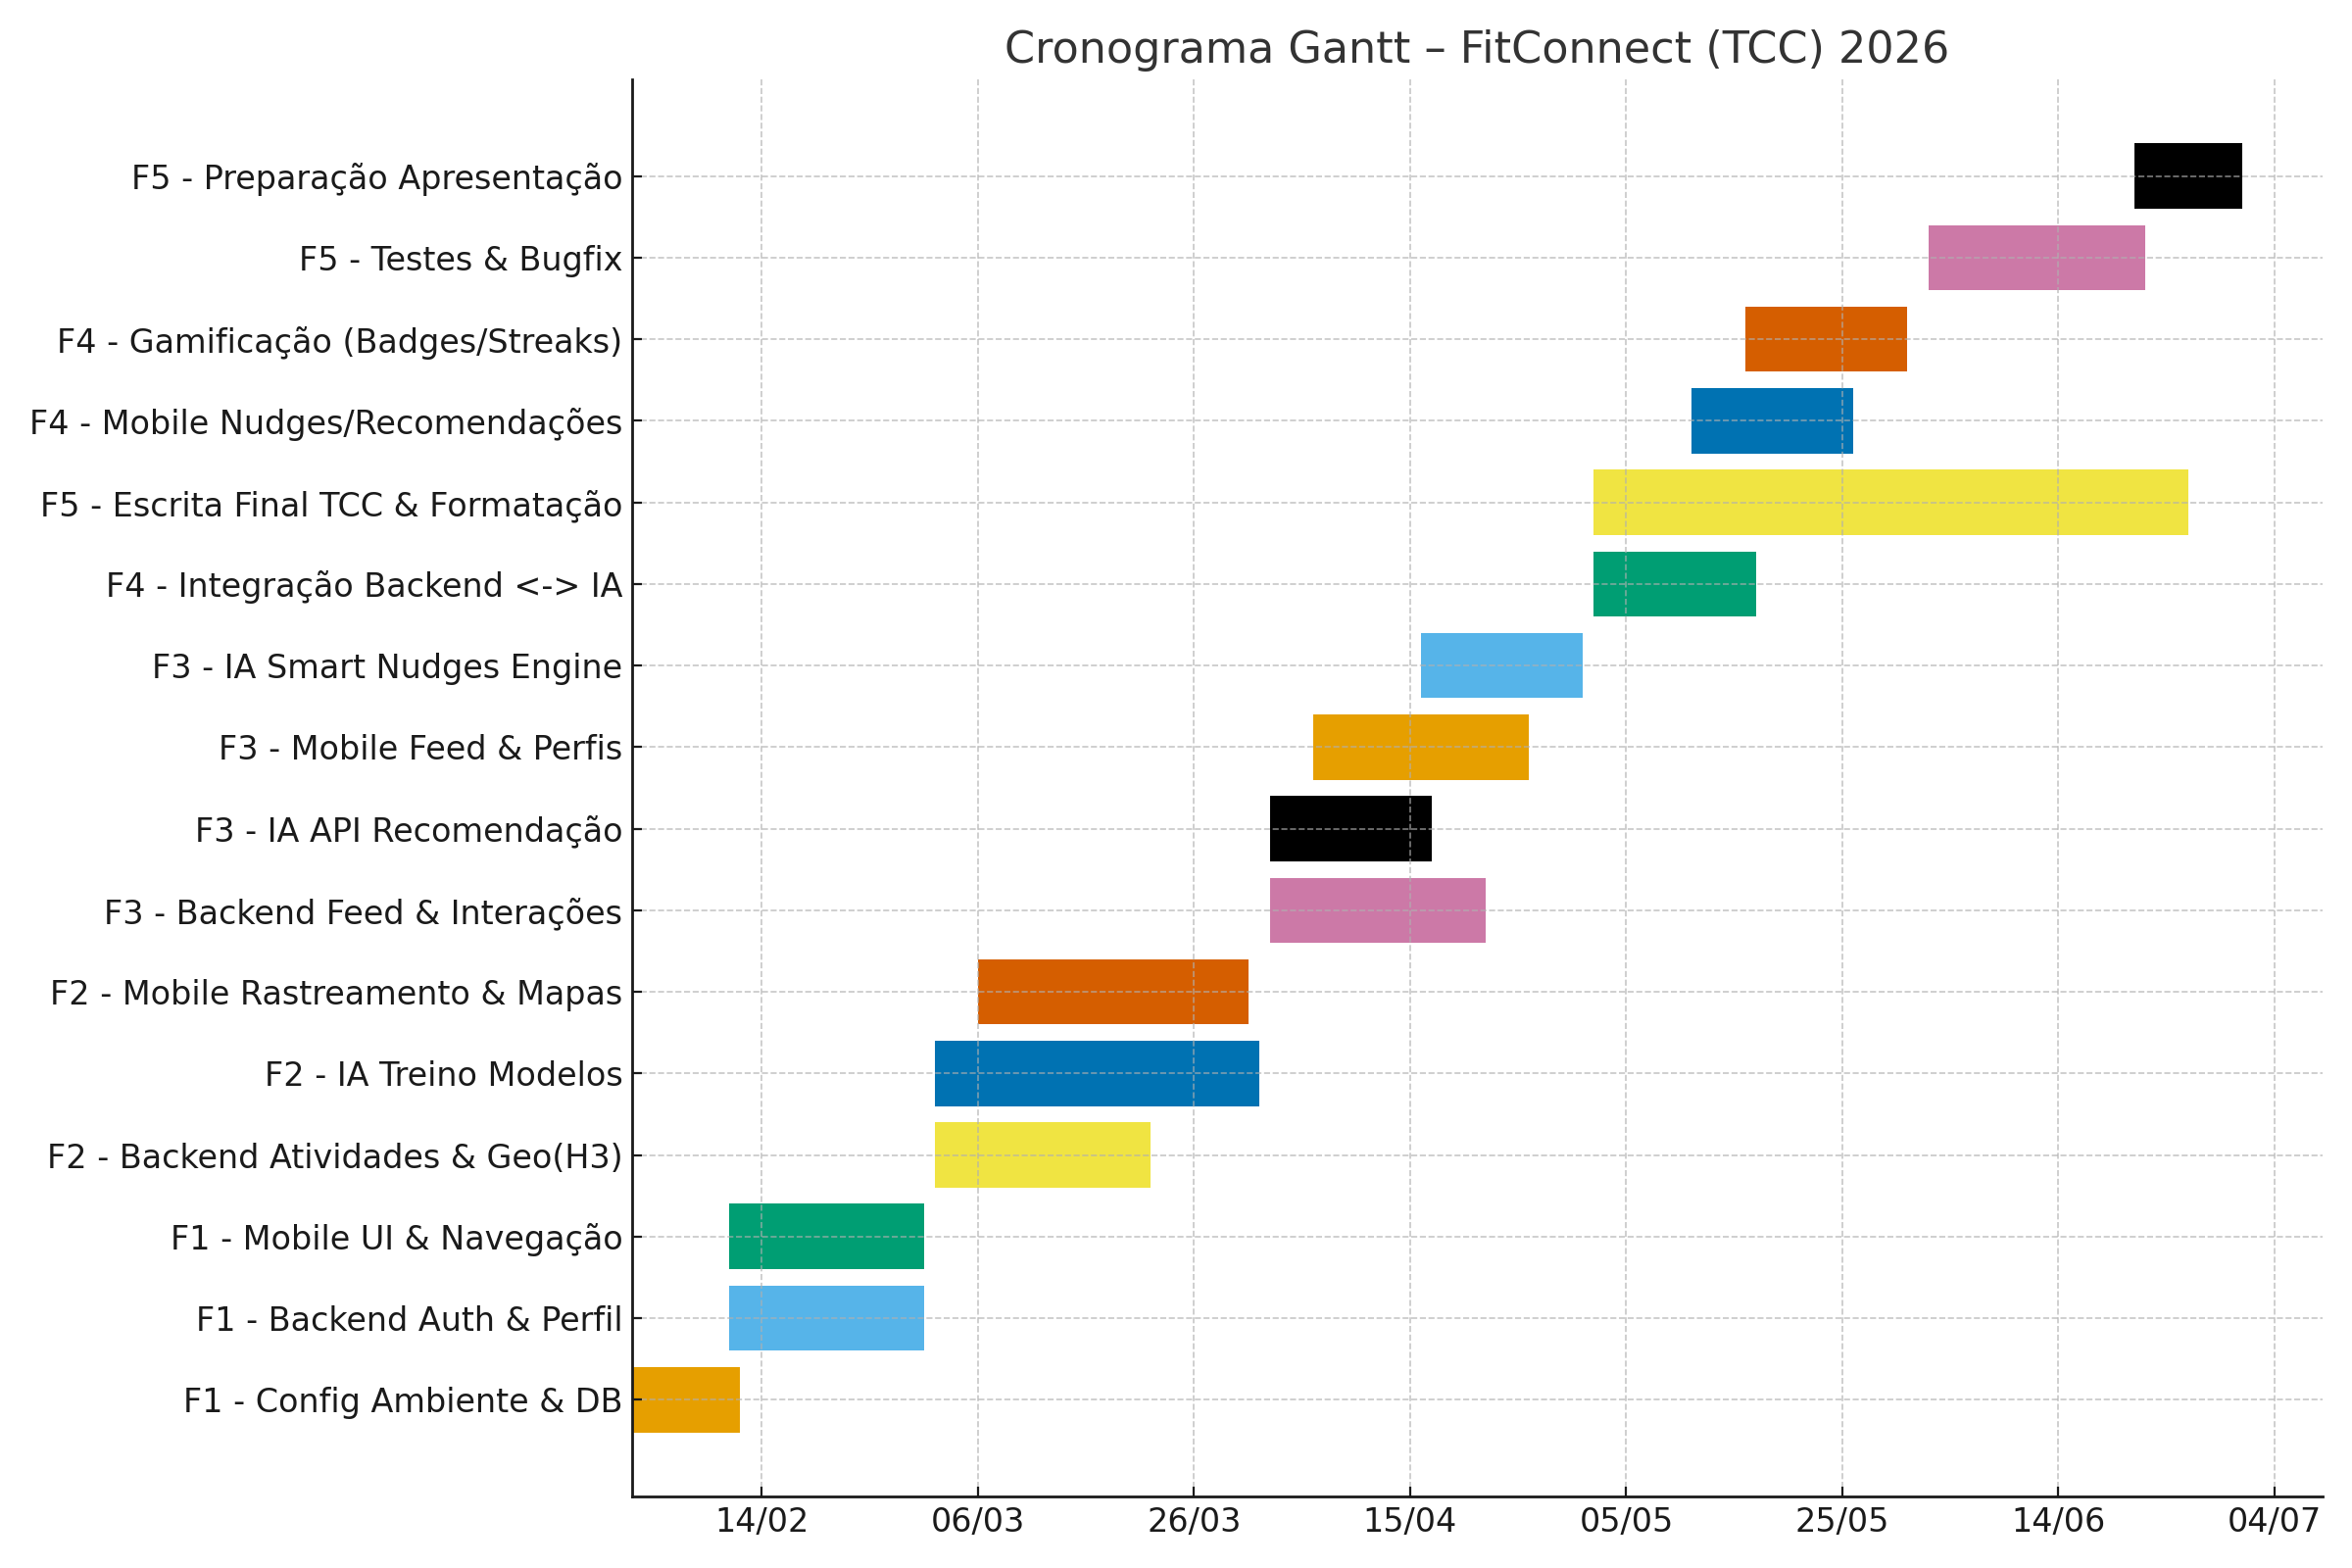
\includegraphics[width=1\textwidth]{figuras/gantt_fitconnect_2026.png}
% \label{fig:gantt}
% \small Fonte: Elaborado pelos autores.
% \end{figure}

% \section{Conclusão}

% \textcolor{green}{Conclusão entra só no TCC2. Pode deixar aqui comentado}

% A implementação do FitConnect surgiu da necessidade de tornar a prática de atividade física mais prática, interativa, inteligente e segura. Foram desenvolvidas, para isso, diferentes tecnologias: um aplicativo para dispositivos móveis com possibilidade de integração a uma pulseira vestível, uma interface web para acompanhamento do progresso e um sistema de recomendação de atividades baseado em Inteligência Artificial (IA). 

% O sistema considera múltiplas características e preferências de cada usuário para construir um perfil detalhado e, a partir dele, gerar um feed personalizado. Entram nesse processo, por exemplo, os tipos de atividades e esportes que a pessoa gosta de praticar, sua idade, peso, nível de condicionamento físico, disponibilidade na rotina e localização geográfica. Com base nesses dados, o FitConnect consegue sugerir conteúdos, treinos e desafios mais alinhados ao perfil individual, aumentando tanto o engajamento quanto a aderência às práticas recomendadas.

% (Nesse paragrafo falar um pouco das limitações que encontramos no projeto)

% (Nesse paragrafo falar dos resultados obtidos nos testes com a IA)

% Entretanto, ainda que o FitConnect seja um aliado muito importante na rotina de cada usuário, o acompanhamento com profissionais da área, como nutricionistas e professores de educação física, continua sendo essencial. A atuação desses especialistas garante maior precisão nas orientações, segurança na realização das atividades e melhores resultados em relação aos objetivos individuais, promovendo uma integração equilibrada entre tecnologia e cuidado humano.
\newpage

\bibliographystyle{abntex2-alf}
\bibliography{bibliografia}

\end{document}